%========================================
% Plantilla artículo - Humanidades Digitales / NLP
% Compilar con: pdfLaTeX + BibTeX + pdfLaTeX + pdfLaTeX
%========================================
\documentclass[11pt,a4paper]{article}

% --- Codificación y tipografía ---
\usepackage[utf8]{inputenc}   % Si usas LuaLaTeX/XeLaTeX, quita inputenc y usa fontspec
\usepackage[T1]{fontenc}
\usepackage{lmodern}
\usepackage{microtype}

% --- Idioma ---
\usepackage[spanish,es-tabla]{babel}  % "Tabla" en lugar de "Cuadro", etc.
\usepackage{csquotes}

% --- Diseño de página ---
\usepackage[margin=1in]{geometry}
\usepackage{setspace}
%\onehalfspacing  % Activa si quieres interlineado 1.5

% --- Matemáticas y figuras/tablas ---
\usepackage{amsmath,amssymb}
\usepackage{graphicx}
\usepackage{booktabs}
\usepackage{tabularx}
\usepackage{siunitx}
\usepackage{longtable}
\usepackage{array}


% --- Hipervínculos y referencias cruzadas ---
\usepackage[hidelinks,colorlinks=true,linkcolor=blue,citecolor=blue,urlcolor=blue]{hyperref}
\usepackage[nameinlink,capitalise,noabbrev]{cleveref}
\usepackage{float}
\usepackage{subcaption}

% --- Bibliografia ----
\usepackage[round,authoryear]{natbib}
\bibliographystyle{apalike}



% --- Comandos útiles ---
\newcommand{\keywords}[1]{\par\noindent\textbf{Palabras clave —} #1}
\newcommand{\JEL}[1]{\par\noindent\textbf{Clasificación —} #1}
\newcolumntype{P}[1]{>{\centering\arraybackslash}p{#1}}


% --- Metadatos ---
\title{Ciencia en la esfera pública de Colombia: \\
	Análisis del discurso en columnas de opinión con metodologías de humanidades digitales y procesamiento de lenguaje natural}

\author{
	Karen Melissa Gomez Montoya\\
	Biviana Marcela Suárez Sierra\\
	\small Universidad EAFIT, Medellín, Colombia\\
	\small \texttt{tu-email@eafit.edu.co}
}

\date{\today}

%========================================
\begin{document}
	\maketitle
	
	\begin{abstract}
		
	\end{abstract}
	
	\keywords{Humanidades digitales; Análisis del discurso; Procesamiento del lenguaje natural; Opinión pública; Colombia}
	

	\section{Introduction}
	
	Science occupies a central position in contemporary public debates. Decisions related to health, the environment, the economy, or education rely on scientific and technological knowledge with the aim of promoting collective well-being and addressing complex problems that affect humanity, such as the development and distribution of vaccines \cite{Chakravartty2022}. In this context, the ways in which science, scientists, and scientific organizations are mentioned, represented, and perceived in media discourse play a key role in shaping public opinion and in legitimizing policies and collective actions \cite{Mede2022}.
	
	Discussions about science in the public sphere have frequently focused on the level of societal trust in science and in scientists (\cite{Cologna2025, Sturgis2021, Mede2022}), as well as on issues related to science communication, outreach, and dissemination. To a lesser extent, research has examined the broader perceptions that different communities hold about science, typically through public opinion surveys.
	
	In Latin America, and particularly in Colombia, these perceptions have been studied primarily through national surveys. In the Colombian case, three such measurements have been conducted: the first in 1994, followed by one in 2004 and another in 2012, the latter administered by the Observatorio Colombiano de Ciencia y Tecnología \cite{Daza_Caicedo2014}. For the organizations that constitute the Science, Technology, and Innovation (STI) ecosystem, both at the national and regional levels, monitoring these public perceptions is essential. Understanding what Colombians think about science makes it possible to improve processes of social appropriation of knowledge, guide political and academic agendas, evaluate communication strategies, and identify the social imaginaries circulating in the public sphere around scientific activity \cite{Daza_Caicedo2014}.
	
	However, beyond surveys, the media represent a privileged arena for observing how science is discursively articulated in the public sphere. Opinion columns, in particular, have been shown to possess the capacity to influence and reshape readers’ perceptions and attitudes, both among elites and the general public \cite{Coppock2018}. At times, scientists themselves turn to this format to intervene in public debate. Nevertheless, previous studies suggest that when writing opinion columns, scientists often lack sufficient rhetorical resources to persuade readers holding divergent positions, tending instead to address audiences who already share similar views \cite{Syfert2025}.
	
	Opinion columns frequently address issues of high scientific and social relevance, such as vaccines, the environment, or climate change. In the Colombian context, this genre has been characterized by a strong argumentative and persuasive orientation, as well as by its focus on current affairs, where the primary objective is to convince the reader \cite{CaroLopera2020}. Despite this, little is still known about how science is discursively integrated into this type of text and with which actors, organizations, topics, and events it is associated.
	

	Against this backdrop, the present study analyzes a sample of approximately 13,000 opinion columns published in three widely circulated Colombian print media outlets, in order to address the following research question: with which topics, organizations, actors, and events is science associated in opinion discourse in Colombia, and what discursive patterns emerge from these associations? To this end, the article proposes a strategy grounded in natural language processing techniques that enables the identification of explicit references to science within the corpus and the examination of their co-occurrences with entities, actors, and domain-specific vocabulary. The aim is to better understand how science is constructed and represented within the Colombian public sphere.
	
	\section{Methodology}
	
	To address the proposed research question, text mining and natural language processing (NLP) methods were employed. The methodology was structured into three main stages. First, references to science were identified within the opinion columns in order to construct a subcorpus. Second, algorithms were applied to analyze authorship, actors, topics, and vocabulary in both the subcorpus and the full corpus, enabling comparative analysis. Finally, the extracted elements were interpreted in light of national events occurring during the publication periods of the opinion columns, and the affiliations of both authors and referenced actors were identified to enrich the analysis. The overall procedure is summarized in the flowchart presented in Figure \ref{fig:diagramaflujo} and is described in detail in the following section. All analyses were conducted using Python 3.12.7 \cite{python3127}, available at \url{https://www.python.org/downloads}.
	
	
	\begin{figure}[H]
		\centering
		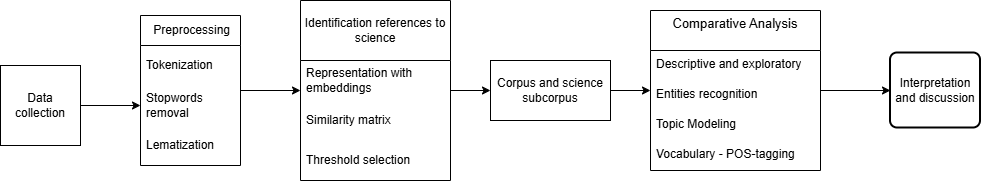
\includegraphics[width=\textwidth]{figures/diagrama_paper_ciencia.png}
		\caption{Flowchart of the applied methodology.}
		\label{fig:diagramaflujo}
	\end{figure}
	
	\subsection{Data collection}
	A total of 13,000 opinion columns were collected from three widely circulated Colombian print media outlets. These columns were published between January 2018 and December 2020. At this stage, the only selection criterion was that the column consist entirely of written text and not require video or audio to understand its content. The columns were not selected based on any specific topic. For each opinion column, the following metadata were collected: the name of the newspaper, the author, the date, the title, the full text (body) of the column, and the URL. Each text was verified to ensure uniqueness (i.e., no duplicated columns), and author names were standardized. After this process, a unique identification number was assigned to each opinion column.
	
	\begin{table}[H]
		\centering
		\caption{Distribution of columns and authors by newspaper}
		\label{tab:col_autores_periodico}
		\footnotesize
		\begin{tabular}{l c c c}
			\hline
			\textbf{Newspaper} & \textbf{Number of columns} & \textbf{Number of distinct authors} & \textbf{\% of total columns} \\
			\hline
			El Espectador & 10509 & 263 & 76.84\\
			El Tiempo & 1982 &  249 & 14.49\\
			Semana & 1185 & 96  & 8.66\\
			\hline
		\end{tabular}
	\end{table}
	
	\subsection{Preprocessing}

		When working with large volumes of text, as in the case of this corpus of opinion columns, analysis cannot begin directly with the raw material. It is first necessary to transform the data into a format that can be interpreted by natural language processing (NLP) algorithms \cite{Chai2022}. This preparatory stage, known as preprocessing, involves a series of methodological decisions aimed at cleaning, structuring, and standardizing the text prior to modeling. In this study, the procedure began with an initial cleaning of each column, during which URLs, hashtags, and social media user mentions (@) were removed, along with redundant whitespace and characters other than letters, numbers, and standard punctuation marks. This cleaning stage reduced noise and helped homogenize the corpus.

		Once cleaned, the text was segmented into basic analytical units through tokenization. This step consists of dividing the text into smaller fragments (known as tokens), which in this case correspond to individual words \cite{Tyagi_text}. Thus, a sentence such as “Tokenization is fundamental” is transformed into the sequence “Tokenization,” “is,” and “fundamental.” Although seemingly straightforward, this operation is essential because it converts unstructured text into a computationally manageable structure, enabling the calculation of frequencies, co-occurrences, and other linguistic metrics.
		

		Subsequently, and depending on the specific requirements of each algorithm applied, so-called stopwords were removed. These are highly frequent words that serve grammatical functions (such as articles, prepositions, pronouns, or conjunctions) and, while essential for syntactic coherence, typically contribute little semantic information in tasks such as topic modeling \cite{Siino2024}. In addition to improving the interpretability of the models, their removal reduces the dimensionality of the corpus, which is computationally advantageous. Because stopword lists are language- and context-dependent, the lists used in this study were reviewed and adjusted prior to application, particularly in the stage preceding topic modeling (see Section \ref{sec:topic_model}).
		
	
		Finally, the process included lemmatization, that is, the reduction of words to their canonical or base form. This standardization makes it possible to group morphological variants under a single lexical entry—for example, converting conjugated verbs to the infinitive or transforming plural nouns into the singular—which is crucial for frequency analyses and lexical studies \cite{Orellana2018}. The selection of the lemmatization model required particular attention. In an initial stage, the lemmatizer from the spaCy library in Python was used, whose main advantage is speed; however, limitations in accuracy for Spanish were observed. For this reason, the Stanford Stanza library model \cite{qi2020stanza}, based on neural networks, was ultimately adopted, as it provided greater accuracy in lemma identification. Lemmatization was applied prior to lexical analysis and part-of-speech (POS) tagging, thereby ensuring a more consistent representation of the corpus vocabulary.

	
	\subsection{Identification of references to science}
	
	
To advance the objective of this study—namely, to understand how science is represented in opinion discourse in Colombia—it was necessary to systematically identify references associated with the scientific field within the previously described corpus. To this end, a strategy based on semantic search was designed. Semantic search is an information retrieval method that enables the identification of meaning-based relationships beyond the literal matching of keywords \cite{Wei2022}. Unlike traditional lexical search, this approach retrieves texts according to their conceptual proximity, incorporating phenomena such as synonymy, terminological variation, and semantic affinity among expressions.

The strategy consisted of representing both the corpus of approximately 13,000 columns and the 17 UNESCO Thesaurus categories for Science through embeddings (vector representations that capture the contextual meaning of texts). Each Thesaurus category (conceived as a semantic field grouping representative terms from different scientific areas) was encoded as a semantic query, composed of the set of words and expressions associated with that category. In parallel, the corpus fragments were transformed into comparable vector representations.


Once these vectors were obtained, semantic similarity between each corpus fragment and each of the 17 categories was calculated using cosine similarity—a metric that quantifies the degree of proximity between two vectors in semantic space. This procedure made it possible to estimate, for each text fragment, a set of affinity scores with respect to the different Thesaurus categories. Based on these scores, a similarity ranking was generated, and each fragment was assigned to the category with the highest recorded value.

As a result, it was possible not only to identify which scientific field categories exhibit greater relative presence within the opinion corpus, but also to retrieve specific column fragments classified according to the category with which they display the greatest semantic proximity. These fragments constitute the basis for the subsequent qualitative analysis, in which discursive patterns associated with the scientific areas registering the highest semantic intensity in the Colombian public sphere are examined.
	
\subsubsection{Definition of science: UNESCO thesaurus}

The words used to represent science were those included in the UNESCO Thesaurus. The UNESCO Thesaurus ``is a controlled and structured list of terms for subject analysis and the retrieval of documents and publications in the fields of education, culture, natural sciences, social and human sciences, communication, and information''\cite{unesco_thesaurus_1977}. Its first English version was published in 1977, and it is periodically revised and updated. For the purposes of this study, the list specifically labeled Science, specialized in the natural sciences, was used. The Spanish-language version of this list was employed for the analysis. This list made it possible to approach science through the words that compose it or are used to identify it across different areas. The category comprises 17 subcategories, each containing between 24 and 84 terms. For reference, a table including the first terms of each category is presented in Table \ref{tab:categorias_ciencia}.

{\footnotesize
	\begin{longtable}{p{3.5cm}P{2cm}p{9cm}}
		\caption{UNESCO Thesaurus Science Categories and the First Terms of Each.} \label{tab:categorias_ciencia}\\
		
		\toprule
		\textbf{Subcategory} & \textbf{No. of terms} & \textbf{First 10 terms} \\
		\midrule
		\endfirsthead
		
		\multicolumn{3}{c}{{\bfseries \tablename\ \thetable{} -- continued}} \\
		\toprule
		\textbf{Subcategory} & \textbf{No. of terms} & \textbf{First 10 terms} \\
		\midrule
		\endhead
		
		\midrule \multicolumn{3}{r}{{Continued on the next page}} \\
		\endfoot
		
		\bottomrule
		\endlastfoot
		
		Scientific approach & 50 & Accessibility, Basic sciences, Benchmarking, Calibration, Case studies, Causal analysis, Cause and effect, Comparative analysis, Cross national analysis,  Design \\
		
		Science and research management & 62 & Academies of science, Applied research, Appropriate technology, Automation, Choice of technology, Diffusion of technology, Digital divide, Digital transformation, Economics of science, Engineers \\
		
		Mathematics and statistics & 34 & Algebra, Algorithms, Arithmetic, Calculus, Combinatorial mathematics, Correlation, Data visualization, Equations, Extrapolation, Factor analysis \\
		
		Physical sciences & 56 & Acoustics, Aerodynamics, Atomic structure, Cooling, Cosmic radiation, Crystallography, Diffusion, Electrical properties, Electricity, Electromagnetic waves \\
		
		Chemical sciences & 50 & Acids, Biochemical analysis, Carbon, Carbon dioxide, Chemical analysis, Chemical compounds, Chemical effects, Chemical elements, Chemical kinetics, Chemical processes \\
		
		Space sciences & 24 & Astronomical systems, Astronomy, Astrophysics, Black holes, Celestial mechanics, Cosmic matter, Cosmology, Earth (planet), Galaxies, Gravitation \\
		
		Earth sciences & 61 & Biogeochemistry, Carbonate rocks, Coastal erosion, Continental drift, Desert soils, Earth sciences, Earth's crust, Erosion, Fossils, Gems \\
		
		Geography and oceanography & 84 & Adriatic Sea, Aegean Sea, Antarctic Ocean, Aral Sea, Arctic Ocean, Atlantic Ocean, Baltic Sea, Basins, Bathymetric charts, Bathymetry \\
		
		Meteorology & 34 & Agroclimatology, Antarctic regions, Arctic regions, Arid zones, Atmosphere, Atmospheric circulation, Atmospheric pressure, Bioclimatology, Climate, Climatic data \\
		
		Hydrology & 46 & Aquifers, Brackish water, Drainage, Drainage basins, Drinking water, Ecohydrology, Freshwater, Groundwater, Hydrogeological maps, Hydrogeology \\
		
		Environmental sciences and engineering & 52 & Animal rights, Aquatic environment, Biological control, Botanical gardens, Desalination, Ecological research, Ecology, Energy balance, Energy conservation, Energy consumption \\
		
		Pollution, disasters and safety & 54 & Accident prevention, Accidents, Acid rain, Agricultural wastes, Air pollution, Avalanches, Climate change, Climate change adaptation, Damage, Dangerous materials \\
		
		Natural resources & 53 & Animal behaviour, Animal ecology, Animal migration, Animal resources, Aquatic ecosystems, Biodiversity, Biogas, Biological adaptation, Biomass, Biomass energy \\
		
		Biology & 75 & Ageing, Anatomy, Artificial procreation, Bacteria, Bacteriology, Biochemicals, Biochemistry, Bioethics, Biogenesis, Biological effects\\
		
		Natural sciences & 50 & Algae, Animal diseases, Animal genetics, Animal nutrition, Animal taxonomy, Animals, Anthropology, Aquatic animals, Aquatic plants, Birds \\
		
		Medical sciences & 54 & Acupuncture, Aerospace medicine, Brain research, Clinical medicine, Dentistry, Dietetics, Disease control, Drug control, Drug policy, Drugs \\
		
		Pathology & 40 & AIDS, Albinism, Blindness, Cancer, Cardiovascular diseases, Clinical psychology, Colour blindness, Deaf dumbness, Deafness, Disabilities \\
		
	\end{longtable}
}


	\subsubsection{Embedding model selection}
For this study, a pre-trained embeddings model was selected. This means that the model had been previously developed and trained on large volumes of textual data, enabling it to capture complex semantic relationships without requiring retraining from scratch. This strategy is grounded in the framework of transfer learning, whereby a model trained on a general task can be effectively reused in different contexts \cite{Hosna2022}. In this way, the corpus of opinion columns could be analyzed by leveraging previously acquired linguistic knowledge, thereby reducing computational costs and development time.

The selection of the embeddings model required consideration of several key criteria. First, the model needed to be optimized for semantic similarity tasks, since the central objective was to measure the conceptual proximity between corpus fragments and the UNESCO Thesaurus categories for Science. Second, it had to provide robust support for the Spanish language, given that the analyzed corpus consists of opinion columns published in Colombia. Finally, the model’s size—understood in terms of the number of parameters and memory requirements—was evaluated, ensuring that it did not exceed 500 million parameters in order to maintain computational feasibility.

The final decision was informed by the results of the Massive Multilingual Text Embedding Benchmark (MMTEB), a large-scale comparative evaluation of multilingual embedding models developed by \cite{enevoldsen2025mmtebmassivemultilingualtext}. This benchmark enables the comparison of model performance across tasks such as information retrieval and semantic similarity. Among the evaluated models, one that achieved a strong balance between performance in Spanish, effectiveness in similarity tasks, and moderate size was embeddinggemma-300m, developed by Google \cite{vera2025embeddinggemmapowerfullightweighttext}. This model comprises approximately 300 million parameters and supports a context window of up to 2048 tokens, making it suitable for processing relatively long text fragments without losing semantic coherence.

Once the model was selected, the corpus was prepared for vector encoding. Because opinion columns often address multiple topics within a single text, working with complete documents would hinder the precise identification of references to science. For this reason, each column was divided into fragments (chunks) of approximately 150 words, with a minimum length of 100 words and an overlap of 20 words between consecutive fragments. Establishing a minimum length is important because the segmentation is performed sequentially from the beginning of the text, which may result in a final fragment that is excessively short; when this occurred, the fragment was merged with the preceding one. The overlap between fragments—meaning that each new segment begins several words before the previous one ends—helps preserve contextual continuity and prevents abrupt semantic breaks. Additionally, this procedure ensures that each fragment remains within the model’s maximum token limit.

Subsequently, a representative embedding was computed for each fragment of the corpus. In a parallel manner, for each UNESCO Thesaurus subcategory, a text was constructed by concatenating its corresponding keywords, and an embedding was generated from this combined string. In this way, both the column fragments and the Thesaurus categories were represented within the same vector space.

Finally, semantic similarity between each corpus fragment and each Thesaurus subcategory was estimated by calculating cosine similarity, with the aim of identifying the degree of conceptual proximity between them. The following section provides a more detailed explanation of the mathematical foundations of cosine similarity and its interpretation in the context of this analysis.

	
	\subsubsection{Cosine similarity}
	
	Once both the corpus fragments and the UNESCO Thesaurus subcategories had been represented within the same vector space through embeddings, it was necessary to define a metric to quantify their semantic proximity. The measure used to evaluate similarity between the encoded texts was cosine similarity, one of the most widely employed metrics in information retrieval and natural language processing (\cite{Jurafsky2025}).
	
	In this context, let $\mathbf{u}$ denote the vector corresponding to a fragment (chunk) of an opinion column, and let $\mathbf{v}$ represent the vector associated with one of the 17 UNESCO Thesaurus categories for Science. The cosine similarity between these two vectors is defined as:
		
	\begin{equation}
		\text{sim}_{\cos}(\mathbf{u}, \mathbf{v}) =
		\frac{\mathbf{u} \cdot \mathbf{v}}
		{\lVert \mathbf{u} \rVert , \lVert \mathbf{v} \rVert}
	\end{equation}
		
	where $\mathbf{u} \cdot \mathbf{v}$ denotes the dot product between the vectors, and $\lVert \mathbf{u} \rVert$ and $\lVert \mathbf{v} \rVert$ correspond to their Euclidean norms. This expression computes the cosine of the angle formed by the two vectors in semantic space.
	
	The value of this measure ranges between -1 and 1. A value close to 1 indicates that the vectors point in the same direction (an angle close to 0 degrees), implying high semantic similarity. A value close to 0 indicates orthogonality (an angle close to 90 degrees), that is, the absence of a meaningful semantic relationship. A value close to -1 corresponds to vectors pointing in opposite directions (an angle close to 180 degrees), which in semantic terms would imply opposition or extreme dissimilarity. In practice, when working with embeddings generated by modern language models, values tend to concentrate in the $[0,1]$ range due to the nature of these representations.
		
	In the procedure implemented in this study, for each corpus fragment $\mathbf{u}$, cosine similarity was computed with each of the 17 vectors $\mathbf{v}$ corresponding to the Thesaurus categories. This yielded, for every fragment, a set of 17 semantic affinity scores. The category assigned to a given fragment was the one with the highest similarity value. In this way, each chunk of the opinion columns was classified according to the scientific field with which it exhibits the greatest conceptual proximity.
	

	\subsubsection{Selection threshold}

Once the full corpus of opinion columns had been segmented, a total of $m = 62{,}651$ fragments (chunks) were obtained. Each of these fragments was represented by an embedding and compared with the $n = 17$ vectors corresponding to the UNESCO Thesaurus categories for Science. Accordingly, the index $i$ ranges over the corpus fragments ($i = 1, \dots, 62{,}651$), and the index $j$ ranges over the Thesaurus categories ($j = 1, \dots, 17$).

For each pair $(i,j)$, cosine similarity was computed between the embedding of text fragment $i$ and the embedding of category $j$. This procedure yielded a similarity matrix $\mathbf{S} \in \mathbb{R}^{m \times n}$, defined as:

\begin{equation}
	\mathbf{S} =
	\begin{bmatrix}
		s_{1,1} & s_{1,2} & s_{1,3} & \cdots & s_{1,n} \\
		s_{2,1} & s_{2,2} & s_{2,3} & \cdots & s_{2,n} \\
		s_{3,1} & s_{3,2} & s_{3,3} & \cdots & s_{3,n} \\
		\vdots  & \vdots  & \vdots  & \ddots & \vdots  \\
		s_{m,1} & s_{m,2} & s_{m,3} & \cdots & s_{m,n}
	\end{bmatrix}
\end{equation}

where each element

$$
s_{i,j} = \text{sim}_{\cos}(\text{text }_i, \text{category }_j)
$$


represents the degree of semantic proximity between fragment $i$ and category $j$.

From this matrix, for each fragment $i$, the category with the highest similarity value was identified, that is,

$$
j^*(i) = \arg\max_{j \in \{1,\dots,17\}} s_{i,j}.
$$

However, this assignment criterion implies that every fragment is classified into some category, even when its similarity levels are low in absolute terms. In other words, the relative maximum procedure does not distinguish between fragments that exhibit a substantively meaningful semantic affinity with the scientific field and those whose proximity is weak or merely incidental.


For this reason, a selection threshold was introduced. Let $\tau \in [0,1]$ denote this threshold. A fragment $i$ is considered an effective mention of science only if

$$
\max_{j} s_{i,j} \geq \tau.
$$

Otherwise, the fragment is not classified as a scientific mention, even if it has been assigned a category under the relative maximum criterion. The appropriate definition of this threshold is crucial, as it allows maximizing the distinction between fragments that contain substantive references to the scientific field and those that do not.

To determine an appropriate value for the threshold $\tau$, a manual validation was conducted based on close reading of a sample of fragments. The purpose of this reading was to construct a reference classification that would make it possible to assess whether the fragments automatically identified through cosine similarity as scientific mentions were indeed so from an interpretative standpoint.

As a preliminary step, the empirical distribution of the maximum similarity scores $j^*(i)$ was examined, and it was observed that values below 0.4 tended to correspond to weak semantic associations. Based on this exploratory inspection, 0.4 was set as an initial cutoff point for constructing the validation sample.

Fragments whose maximum similarity score exceeded 0.4 were then filtered. From this subset, 10 fragments were randomly selected for each of the 17 Thesaurus categories, yielding a total of 170 fragments. Each fragment was read and manually classified as either an “effective mention of science” or a “non-mention,” depending on whether its content substantively corresponded to the assigned scientific field.

This manual classification made it possible to compare the automatic assignment with human evaluation. In the automated procedure, each fragment is associated with the category exhibiting the highest similarity $j^*(i)$, but it is considered an effective mention of science only if the maximum similarity value $\max_j s_{i,j}$ exceeds the threshold $\tau$. Accuracy was calculated as the proportion of matches between the manual reference classification and the automatic decision (assignment combined with threshold validation). By evaluating different values of $\tau$, it was possible to identify the point that maximizes agreement between the computational procedure and the interpretative reading.

Figure~\ref{fig:resultados-clasificacion} shows the evolution of accuracy as a function of the threshold $\tau$ used to determine whether a corpus fragment constitutes an effective mention of science. The horizontal axis represents the different possible threshold values, while the vertical axis displays the level of agreement between the automatic classification and the manual reference classification. Each point on the curve corresponds to the accuracy obtained by applying a specific value of $\tau$ to the validation sample. The graph illustrates how model performance varies as the decision criterion becomes more or less stringent.

For example, if the threshold is set at $\tau = 0.47$, a fragment is classified as a scientific mention only when its maximum similarity with one of the 17 Thesaurus categories satisfies
\[
\max_j s_{i,j} \ge 0.47.
\]

Applying this criterion to the 170 manually evaluated fragments yields an accuracy close to 0.74. This means that approximately 74\% of the automatic decisions coincide with the classification obtained through close reading. In practical terms, the model reproduces human judgment in nearly three out of four cases. This value represents a point of balance: if the threshold were lower, weak semantic associations would be included; if it were higher, fragments containing substantive references to science would be excluded.

With the selected threshold, the procedure was applied to the full set of $62{,}651$ corpus fragments, resulting in the identification of a subcorpus composed of $7{,}267$ chunks that meet the criterion of an effective mention of science. This subcorpus constitutes the basis for the subsequent thematic analyses.

	
\begin{figure}[H]
	\centering
	\begin{subfigure}{0.48\textwidth}
		\centering
		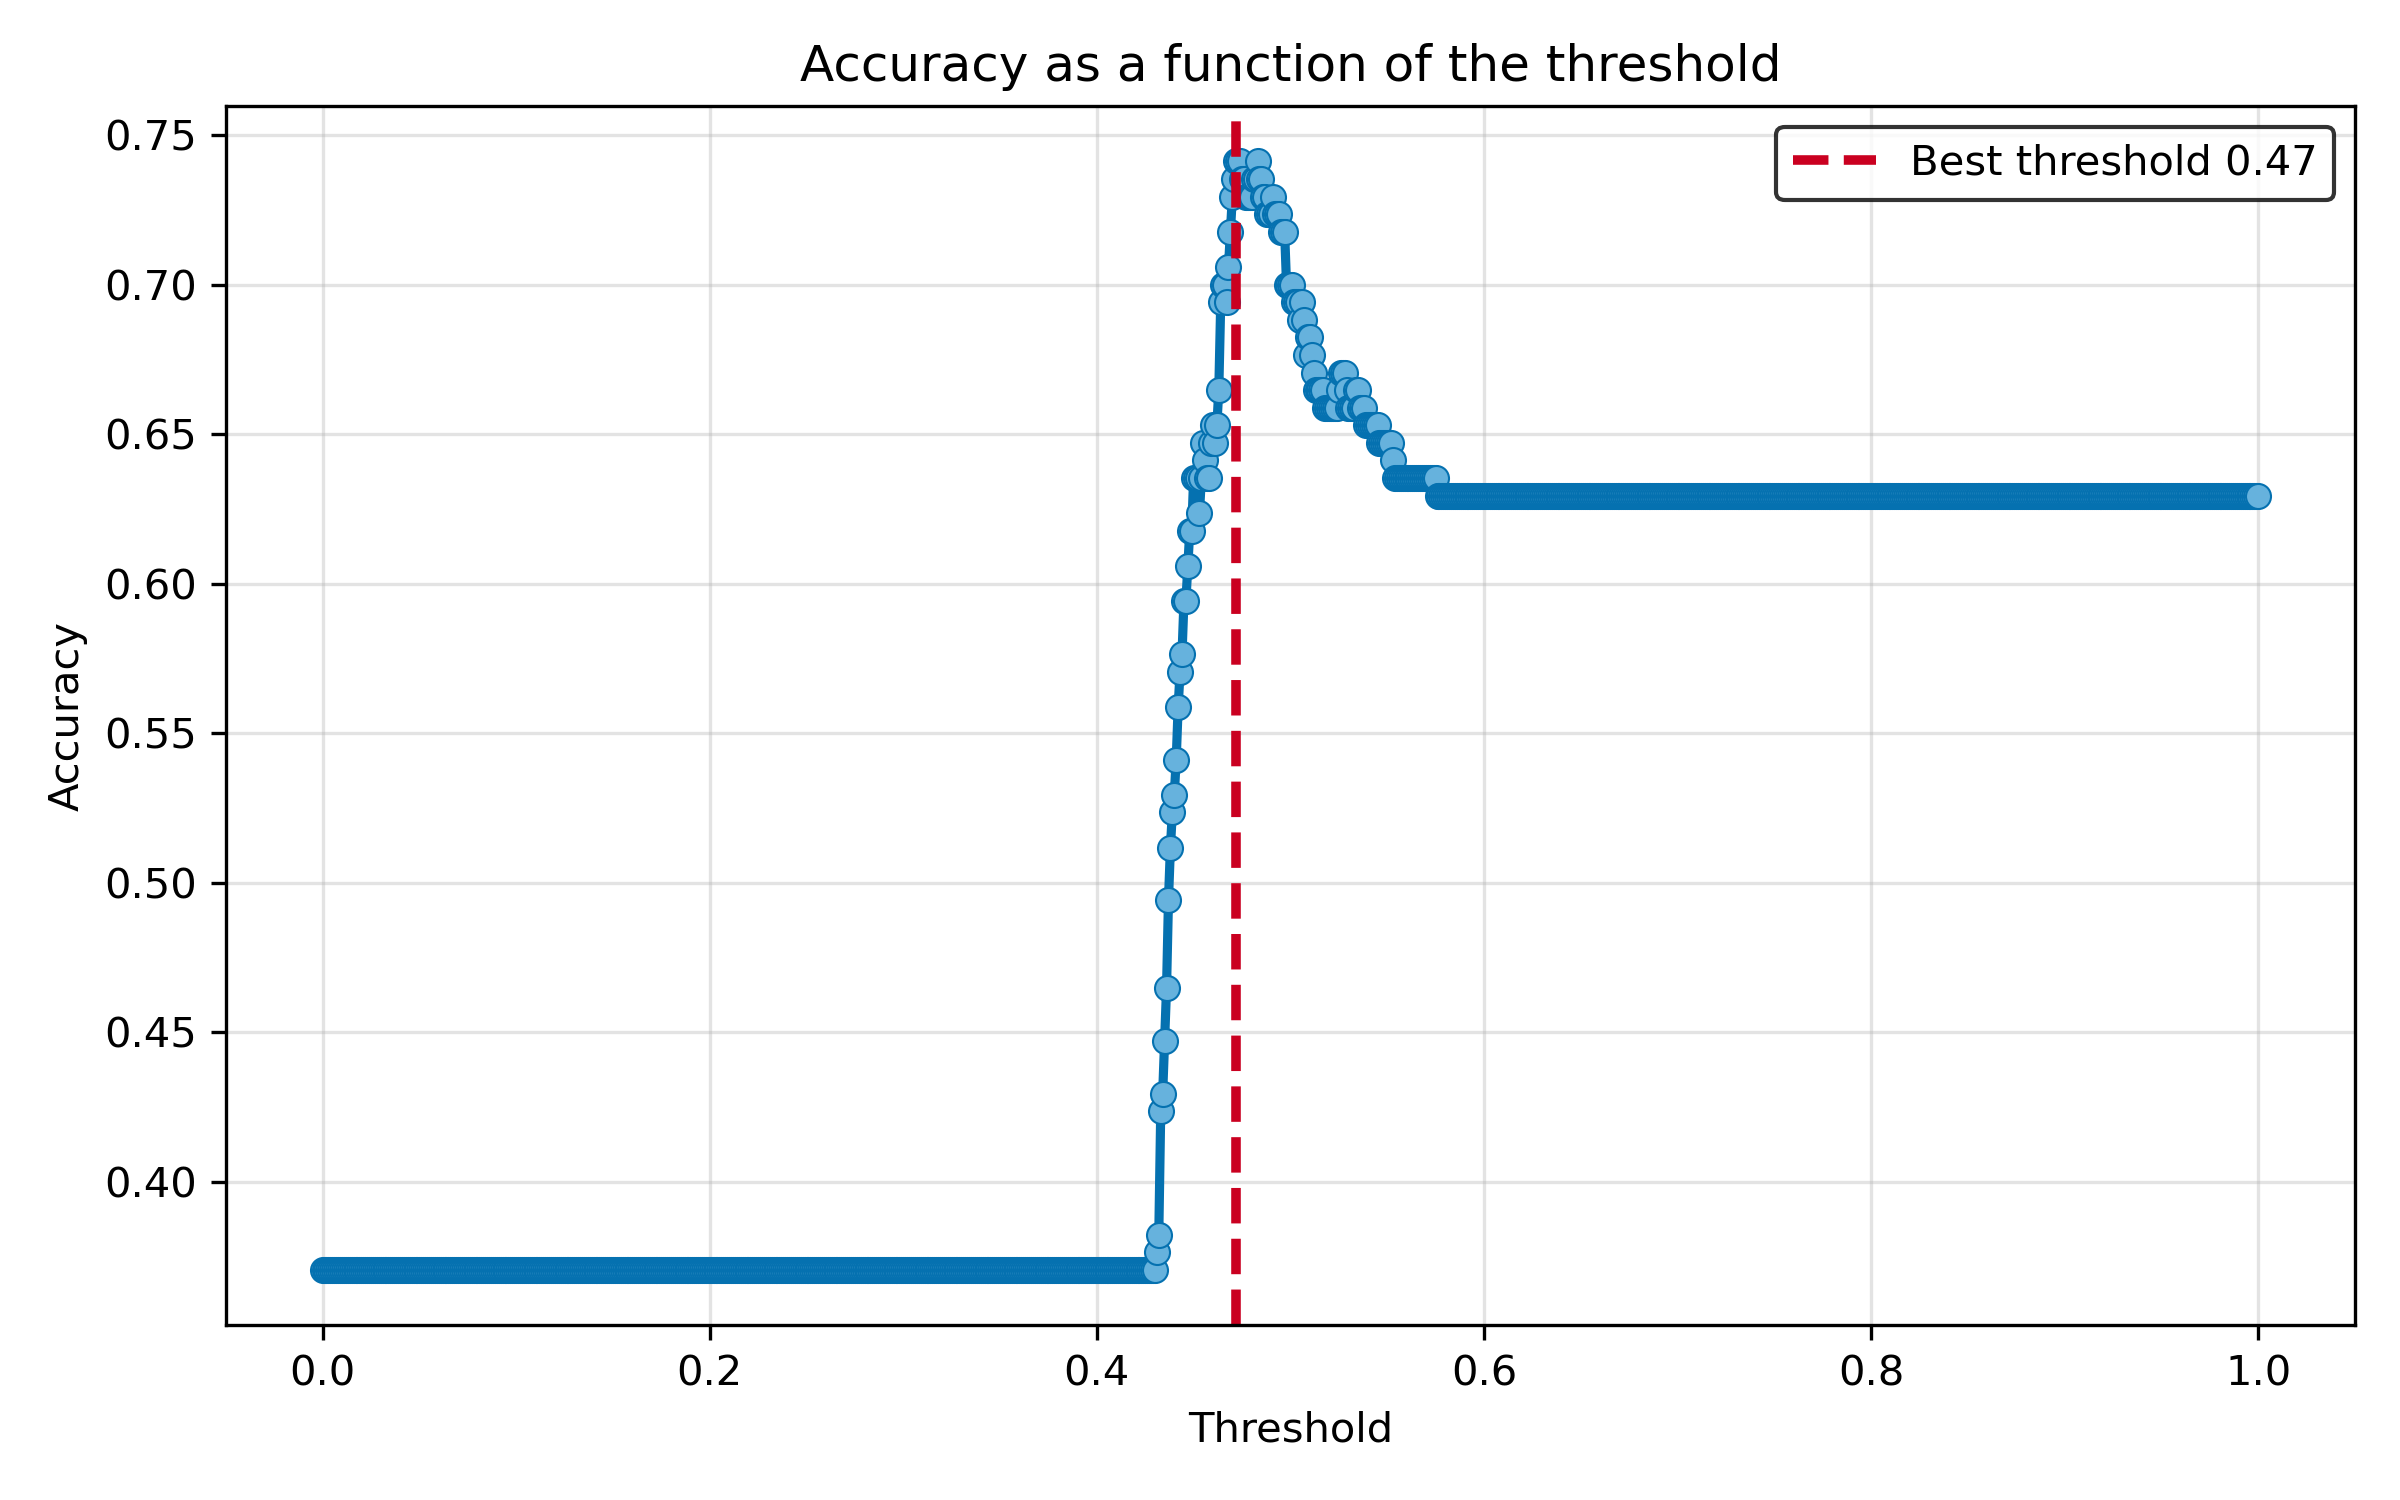
\includegraphics[width=\textwidth]{figures/accuracy_umbral.png}
		\caption{Accuracy by threshold.}
		\label{fig:accuracy-umbral}
	\end{subfigure}
	\caption{Classification analysis results: distribution of scores and accuracy according to threshold.}
	\label{fig:resultados-clasificacion}
\end{figure}


\subsection{Descriptive and exploratory analyses of the text}
	
	
	To characterize the corpus and establish an appropriate foundation for subsequent analyses, a general descriptive procedure was conducted through the calculation of various statistics. These included the total number of words, the number of unique words, as well as the maximum and minimum document length per column. Such indicators make it possible to assess the structure and scope of the text collection prior to advancing toward more specific analyses.
	
	Additionally, in order to obtain an exploratory approximation of the discursive content, two word clouds were generated: one corresponding to the full corpus and another to the science subcorpus. Their construction involved preprocessing steps including text cleaning, normalization, and tokenization. The word clouds were built from term frequencies, facilitating a preliminary comparison of the predominant vocabularies in each dataset.
	
	Finally, a temporal analysis was conducted based on the calculation of the monthly volume of documents and the identification of those containing science-related mentions. This procedure enabled the construction of a chronological series intended to examine the temporal dynamics of thematic presence in subsequent stages of the analysis.
	
	
	
	\subsection{Entity analysis – NER}
	
	
	Named Entity Recognition (NER) is a natural language processing task that consists of identifying entities mentioned in a text and classifying them into predefined categories (e.g., persons, locations, or organizations) \cite{Jehangir2023}. This process plays a fundamental role in a wide range of applications, including social network analysis, semantic annotation, machine translation, question answering systems, automatic text summarization, document classification, spam detection, and opinion mining \cite{Jehangir2023}.
	
	In this study, a named entity recognition model was applied to the entire corpus, followed by a comparative analysis with the science subcorpus. To this end, the frequency of occurrence of each entity was calculated in both corpora, and a ratio was computed to indicate the extent to which a given entity appears more frequently in science-related texts than in the rest of the corpus.
	
	The model used was\textit{ Babelscape/wikineural-multilingual-ner} \cite{tedeschi-etal-2021-wikineural-combined}, available in the Sentence Transformers library. This model exhibits strong performance metrics and is pre-trained on multilingual data that include Spanish. It recognizes locations, persons, and organizations, and groups entities that do not fit these categories into a miscellaneous class.
	
	
	
	\subsection{Analysis of topics}\label{sec:topic_model}
	
	
	Once the science-related mentions had been identified and the corresponding subcorpus constructed, topic modeling was conducted in order to infer the latent thematic structures present in both the general corpus and the science subcorpus. Topic modeling comprises a set of unsupervised methods aimed at discovering recurrent semantic patterns within a collection of documents \cite{Abdelrazek2023}. Conceptually, these methods seek to model three fundamental entities: the document collection, the latent topics, and the constructs that compose them. In this context, the constructs correspond to the lexical units (words or terms) that make up the analyzed fragments.

	From a mathematical standpoint, a topic can be understood as a probability distribution over the vocabulary of the corpus. That is, given a set of words $w_1, w_2, \dots, w_V$ that constitute the vocabulary, a topic $k$ is represented as a probability vector

	$$
	\boldsymbol{\phi}_k = \left( P(w_1 \mid k), P(w_2 \mid k), \dots, P(w_V \mid k) \right),
	$$
	
	donde $P(w_v \mid k) \ge 0$ y
	
	$$
	\sum_{v=1}^{V} P(w_v \mid k) = 1.
	$$
	
	For example, a topic associated with the field of health might assign higher probabilities to terms such as \textit{vaccine}, \textit{epidemic}, \textit{hospital}, or \textit{public health}, while other words in the vocabulary would receive probabilities close to zero. In this way, a topic is not defined by a single word, but rather by a probabilistic structure that describes the relative relevance of terms within that latent theme.
	
	The literature identifies four major families of methods for topic modeling: algebraic, fuzzy, probabilistic, and neural. Algebraic models, which emerged in the 1990s, constituted the first systematic attempts to identify thematic structures through matrix decompositions. More recently, neural approaches have attracted greater attention due to their capacity to capture complex semantic relationships. Among them, BERTopic \cite{Grootendorst2022} stands out, as it combines pre-trained embeddings, dimensionality reduction, and clustering algorithms to identify groups of documents with high semantic proximity.
	
	Since embeddings had already been used in earlier stages of the analysis to represent corpus fragments, methodological coherence was maintained by employing the same vector representation model (embeddinggemma-300m) for topic modeling. This ensures that the semantic structure captured in the identification of scientific mentions is preserved in the subsequent thematic inference.
	
	The model was applied to both the full corpus and the science subcorpus, enabling subsequent comparisons between general thematic configurations and those specifically associated with scientific discourse. The implementation in Python allowed control over various components of the process, including the embeddings model, the maximum number of topics to estimate, and the minimum number of documents required to form a topic. In addition, an outlier reduction procedure was applied to decrease the number of unassigned fragments and enforce a more exhaustive classification.
	
	To evaluate the quality of the estimated topics, the topic coherence metric was used. This measure, based on probabilistic principles of term co-occurrence, has been shown to correlate positively with human interpretability of topics \cite{Rder2015}. In order to select the optimal number of topics, the model was run with different parameter values, and the corresponding coherence was calculated in each case. The value that maximized this metric was adopted as the final configuration of the model.


	\subsection{Vocabulary Analysis with POS-Tagging}
	
	In order to identify the most relevant vocabulary associated with scientific discourse in opinion columns, a frequency analysis of verbs, adjectives, and nouns was conducted for both the general corpus and the science subcorpus. To obtain these grammatical categories, a Part-of-Speech Tagging (POS-tagging) model was employed. This task consists of assigning each word its corresponding syntactic category (noun, verb, adjective, preposition, among others) \cite{he2020surveyrecentadvancessequence}. POS-tagging constitutes a fundamental component in various natural language processing applications, such as machine translation, information retrieval and extraction, syntactic parsing, semantic disambiguation, and sentiment analysis \cite{Chiche2022}.
	
	For this study, the Stanza POS-tagger was used. Stanza is a Python-based linguistic analysis package that includes models trained for multiple languages, including Spanish \cite{qi2020stanzapythonnaturallanguage}. This model was selected due to its reported performance metrics and its suitability for journalistic texts. In the analyzed corpus, it exhibited consistent behavior, enabling the reliable extraction of the grammatical classes required for the comparative frequency analysis.
	
	
	
	\section{Results}


In this section, the results derived from the methodological procedure described above are presented, following the same analytical sequence. First, the identification of effective mentions of science and the delimitation of the corresponding subcorpus are reported. Subsequently, descriptive and exploratory analyses are presented to quantitatively characterize its presence within the corpus. Next, the results of the named entity recognition task are introduced in order to identify actors and institutions associated with scientific discourse. This is followed by the findings of the topic modeling, which allow the inference of latent thematic structures in both the general corpus and the science subcorpus. Finally, lexical and grammatical patterns are analyzed through POS-tagging techniques, contributing to a more detailed understanding of the linguistic form adopted by the representation of science in the public sphere.


	
\subsection{Identification of Mentions of Science}\label{sec:ident_menciones}


Based on the manual classification of 170 fragments used for validation, an appropriate threshold was determined to be $\tau = 0.47$, yielding an \emph{accuracy} of 0.741. Once this criterion was established, the procedure was applied to the full set of 13,676 opinion columns, which had been segmented into 62,651 fragments. Of these, 7,267 fragments were identified as related to science, representing 11.6\% of the total number of fragments.


At the document level, 4\,154 columns contain at least one effective mention of science, corresponding to 30.4\% of the total number of analyzed columns. Table~\ref{tab:res_fragmentos_subcategoria} presents the distribution of fragments classified as scientific mentions across the 17 categories of the UNESCO Thesaurus.

	
	
	{\footnotesize
		\begin{longtable}{p{7cm}P{4cm}P{4cm}}
			\caption{Number of fragments with mentions of science and percentage of the total by category} \label{tab:res_fragmentos_subcategoria}\\
			\toprule
			\textbf{Subcategory} & \textbf{Number of fragments} & \textbf{Percentage of total} \\
			\midrule
			\endfirsthead
			
			\multicolumn{3}{c}{{\bfseries \tablename\ \thetable{} -- continued}} \\
			\toprule
			\textbf{Category} & \textbf{Number of fragments} & \textbf{Percentage of total} \\
			\midrule
			\endhead
			
			\midrule \multicolumn{3}{r}{{Continued on the next page}} \\
			\endfoot
			
			\bottomrule
			\endlastfoot
			
			Administration of science and research & 3195 & 43.97\% \\
			Pollution, disasters and safety & 1566 & 21.55\% \\
			Environmental sciences and engineering & 635 & 8.74\% \\
			Natural sciences & 470 & 6.47\% \\
			Pathology & 375 & 5.16\% \\
			Medical sciences & 306 & 4.21\% \\
			Mathematics and statistics & 250 & 3.44\% \\
			Hydrology & 104 & 1.43\% \\
			Natural resources & 68 & 0.94\% \\
			Scientific approach & 64 & 0.88\% \\
			Space sciences & 61 & 0.84\% \\
			Geography and oceanography & 49 & 0.67\% \\
			Biology & 36 & 0.50\% \\
			Meteorology & 28 & 0.39\% \\
			Earth sciences & 23 & 0.32\% \\
			Physical sciences & 20 & 0.28\% \\
			Chemical sciences & 17 & 0.23\% \\
			\midrule
			\textbf{Total} & \textbf{7267} & \textbf{100\%} \\
		\end{longtable}
	}
	
	
	 
	
	A  continuación se incluyen algunos ejemplos de los fragmentos seleccionados. \textcolor{green}{Poner los originales en material suplementario, acá se ponen los traducidos al inglés, si no has visto en la revisión de la literatura una mejor opción de mostrarlos, además deberíamos compartir el enlace de donde los tomamos y mencionar la línea en donde empieza y donde termina la referencia en el texto original}\\
	 
	
	De la categoría: Administración de la ciencia y de la investigación
	
	\begin{quote}
		(...) separado. El Ministerio de Ciencia, Tecnología e Innovación tiene la responsabilidad de convocar la constitución de un Sistema Nacional de Innovación que asuma como propósito desarrollar la hoja de ruta planteada por la Misión de Sabios, alineando a todos los actores a nivel local, regional y nacional. El conocimiento siempre es un logro colectivo. Frente a los desafíos que afrontamos como país, es necesario que asumamos colectivamente, todos los actores, el reto de gestionar el conocimiento, aprendiendo de manera continua, para ponerlo al servicio de las comunidades. Para superar la crisis y lograr las transformaciones estructurales se requiere planeación y un trabajo de mediano y largo plazo, en donde todos sumemos sin pensar solo en réditos inmediatos. Un sistema en donde el arte, las humanidades, la tecnología y las ciencias sociales y exactas, como expresión del conocimiento, hagan parte de la cotidianidad de los colombianos nos exige dejar de actuar (...)
	\end{quote}
	
	De la categoría Ciencias ambientales e ingeniería
	
	\begin{quote}
		(...) la justicia ambiental y climática. 4. Articular los objetivos de desarrollo sostenible y la agenda 2030 del posconflicto, focalizándonos en energías renovables, transporte multimodal, bioconstrucción, permacultura, autoconsumo y territorios hídricos resilientes. 5. Redefinir la relación urbanorural, enfatizando restauración y conservación de ecosistemas, equidad, solidaridad, corresponsabilidad e identidad. 6. Revisar el modelo mineroenergético ajustándolo al ordenamiento ambiental territorial, no construir nuevos megaproyectos hidroeléctricos, negar el uso del fracking y hacer transición energética hacia energías renovables alternativas. 7. Promover la educación integral y la democratización de la información y el conocimiento como instrumentos de construcción de la paz, respetando las utopías y las diversidades culturales y naturales. 8. Fortalecer la investigación científica, la innovación y otros modos de construcción del conocimiento como medios para mejorar el conocimiento de la realidad ecológica, climática y cultural. 9. Reconocer a la naturaleza como víctima del conflicto armado y del modelo de desarrollo colombiano, y, por (...)
	\end{quote}
	
	De la categoría Matemáticas y estadística
	
	\begin{quote}
		(...) la ciencia aspira a los modelos económicos, a reducirlo todo a un cuerpo teórico pequeño de donde se puedan desprender, por deducción directa, sus corolarios básicos. En matemáticas, digamos, es más bella una demostración corta y aritmética que otra más larga que deba recurrir al cálculo para demostrar lo mismo. Todas las geometrías se desarrollan a partir de un puñado de postulados elementales. Los físicos sueñan con la Teoría del Todo están hartos de lidiar con ese enjambre de partículas empalagosas. ¡Eso no es elegante!. En ciencia, como en arte, lo bello es lo breve, lo simple, así haya siempre una secreta complejidad escondida entre los pliegues. Sí, dedicaré lo mejor de mis días a la búsqueda de la fragancia madre y cuando la encuentre la envasaré en un frasquito que será una gema discreta, claro, y la pondré a los pies de mi esposa, lo prometo. El resto será (...)
	\end{quote}
	
	De la categoría Ciencias químicas
	
	\begin{quote}
		(...) a la formación en ciencias de la naturaleza sabemos que el conocimiento científico y tecnológico tiene unos efectos sociales, económicos y políticos que se deben analizar rigurosamente para que nuestros estudiantes fundamenten su formación ciudadana de manera amplia y crítica, de tal manera que cuenten con las herramientas conceptuales y metodológicas para participar activamente en la vida social. Por ejemplo, cuando estudiamos el tema de hidrocarburos, no solo debemos entender su disposición en la naturaleza, sus propiedades y estructuras químicas, sino también analizar su importancia social, los procesos de explotación y los usos sociales que, en su mayoría, están asociados a la generación de energía a partir de la mezcla de hidrocarburos más famosa que conocemos en el mundo y que denominamos petróleo; al estudiar este tema no solo debemos comprenderlo científicamente, sino considerar simultáneamente que esta mezcla de sustancias orgánicas representa el componente central de la matriz energética del (...)
	\end{quote}
	
	
	
\subsection{Descriptive and Exploratory Analyses}

	
	\begin{table}[H]
		\centering
		\caption{Estadísticos descriptivos generales del corpus}
		\label{tab:estadisticos_generales}
		\begin{tabular}{l c}
			\hline
			\textbf{Estadístico} & \textbf{Valor} \\
			\hline
			Número total de documentos & 13676\\
			Palabras totales & 8607473\\
			Promedio palabras por documento & 629\\
			Mediana palabras por documento & 590\\
			Máximo palabras por documento & 5223\\
			Mínimo palabras por documento & 128\\
			Número de autores distintos & 584\\
			Número de medios de comunicación distintos & 3\\
			Número de palabras únicas (vocabulario total) & 283923\\
			\hline
		\end{tabular}
	\end{table}
	
		\begin{figure}[H]
		\centering
		\begin{subfigure}{0.48\textwidth}
			\centering
			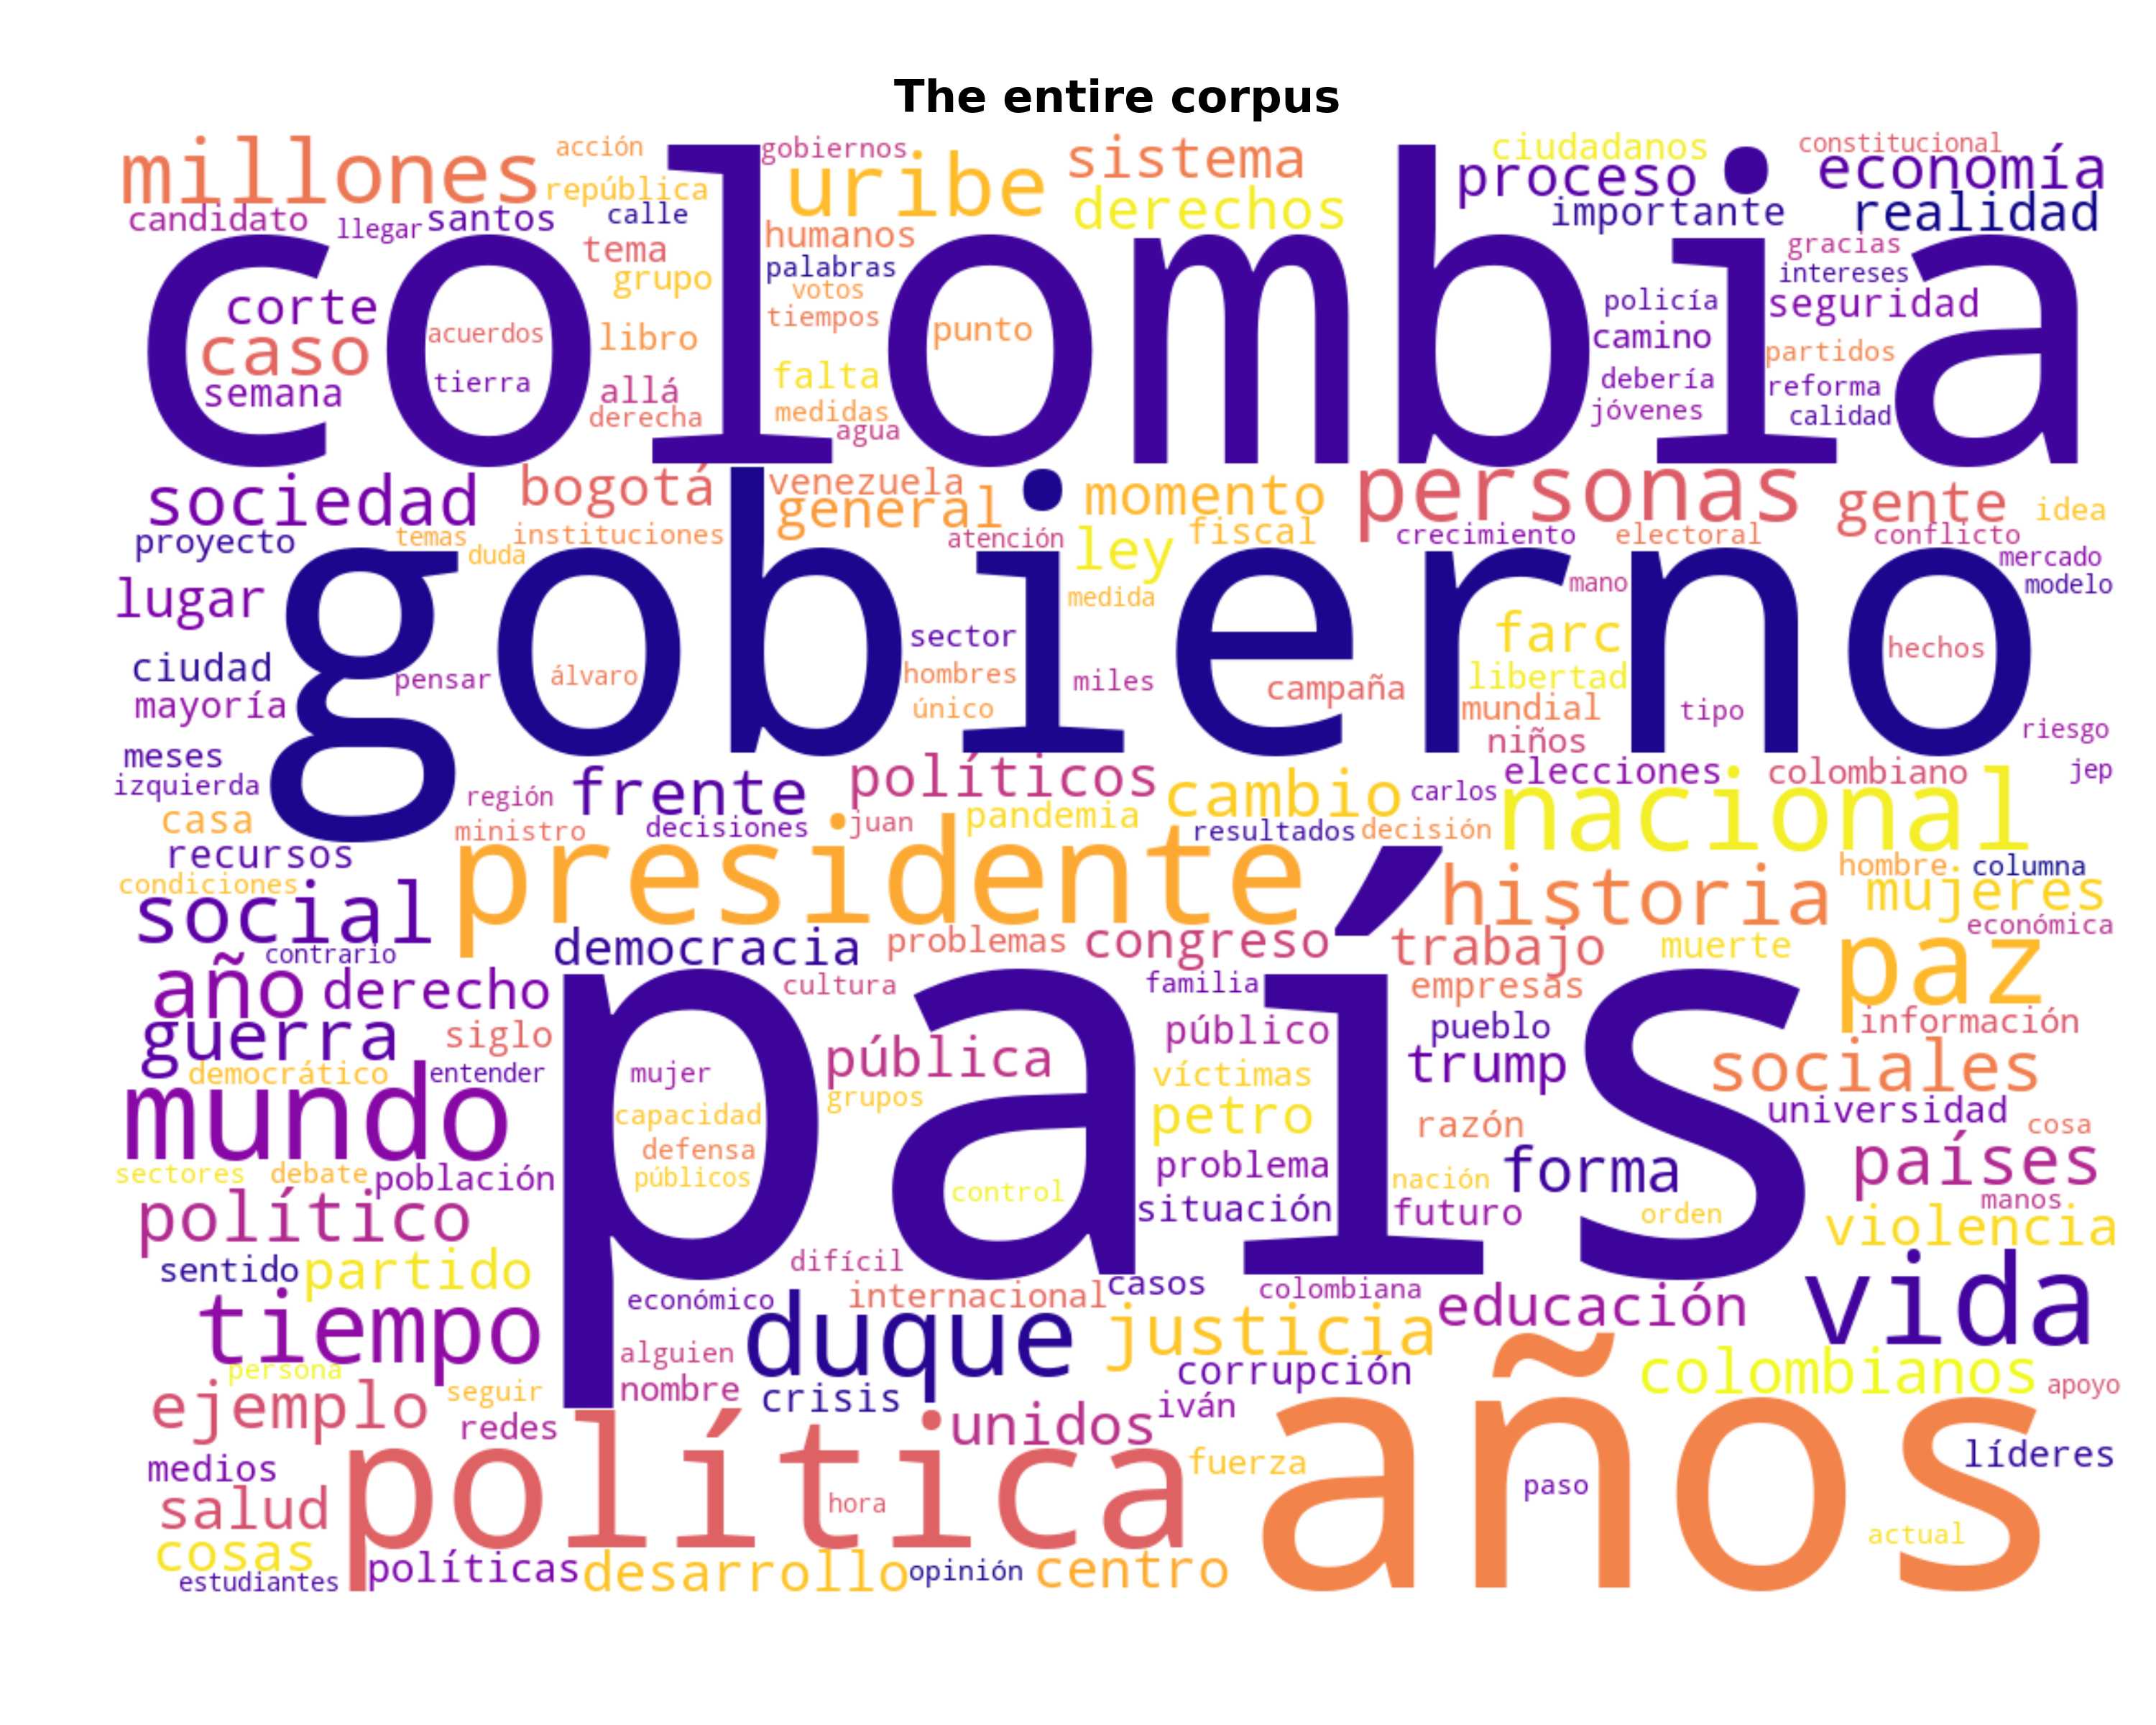
\includegraphics[width=\textwidth]{figures/nube_general.png}
			\caption{Nube de palabras corpus general}
			\label{fig:nube_general}
		\end{subfigure}
		\hfill
		\begin{subfigure}{0.48\textwidth}
			\centering
			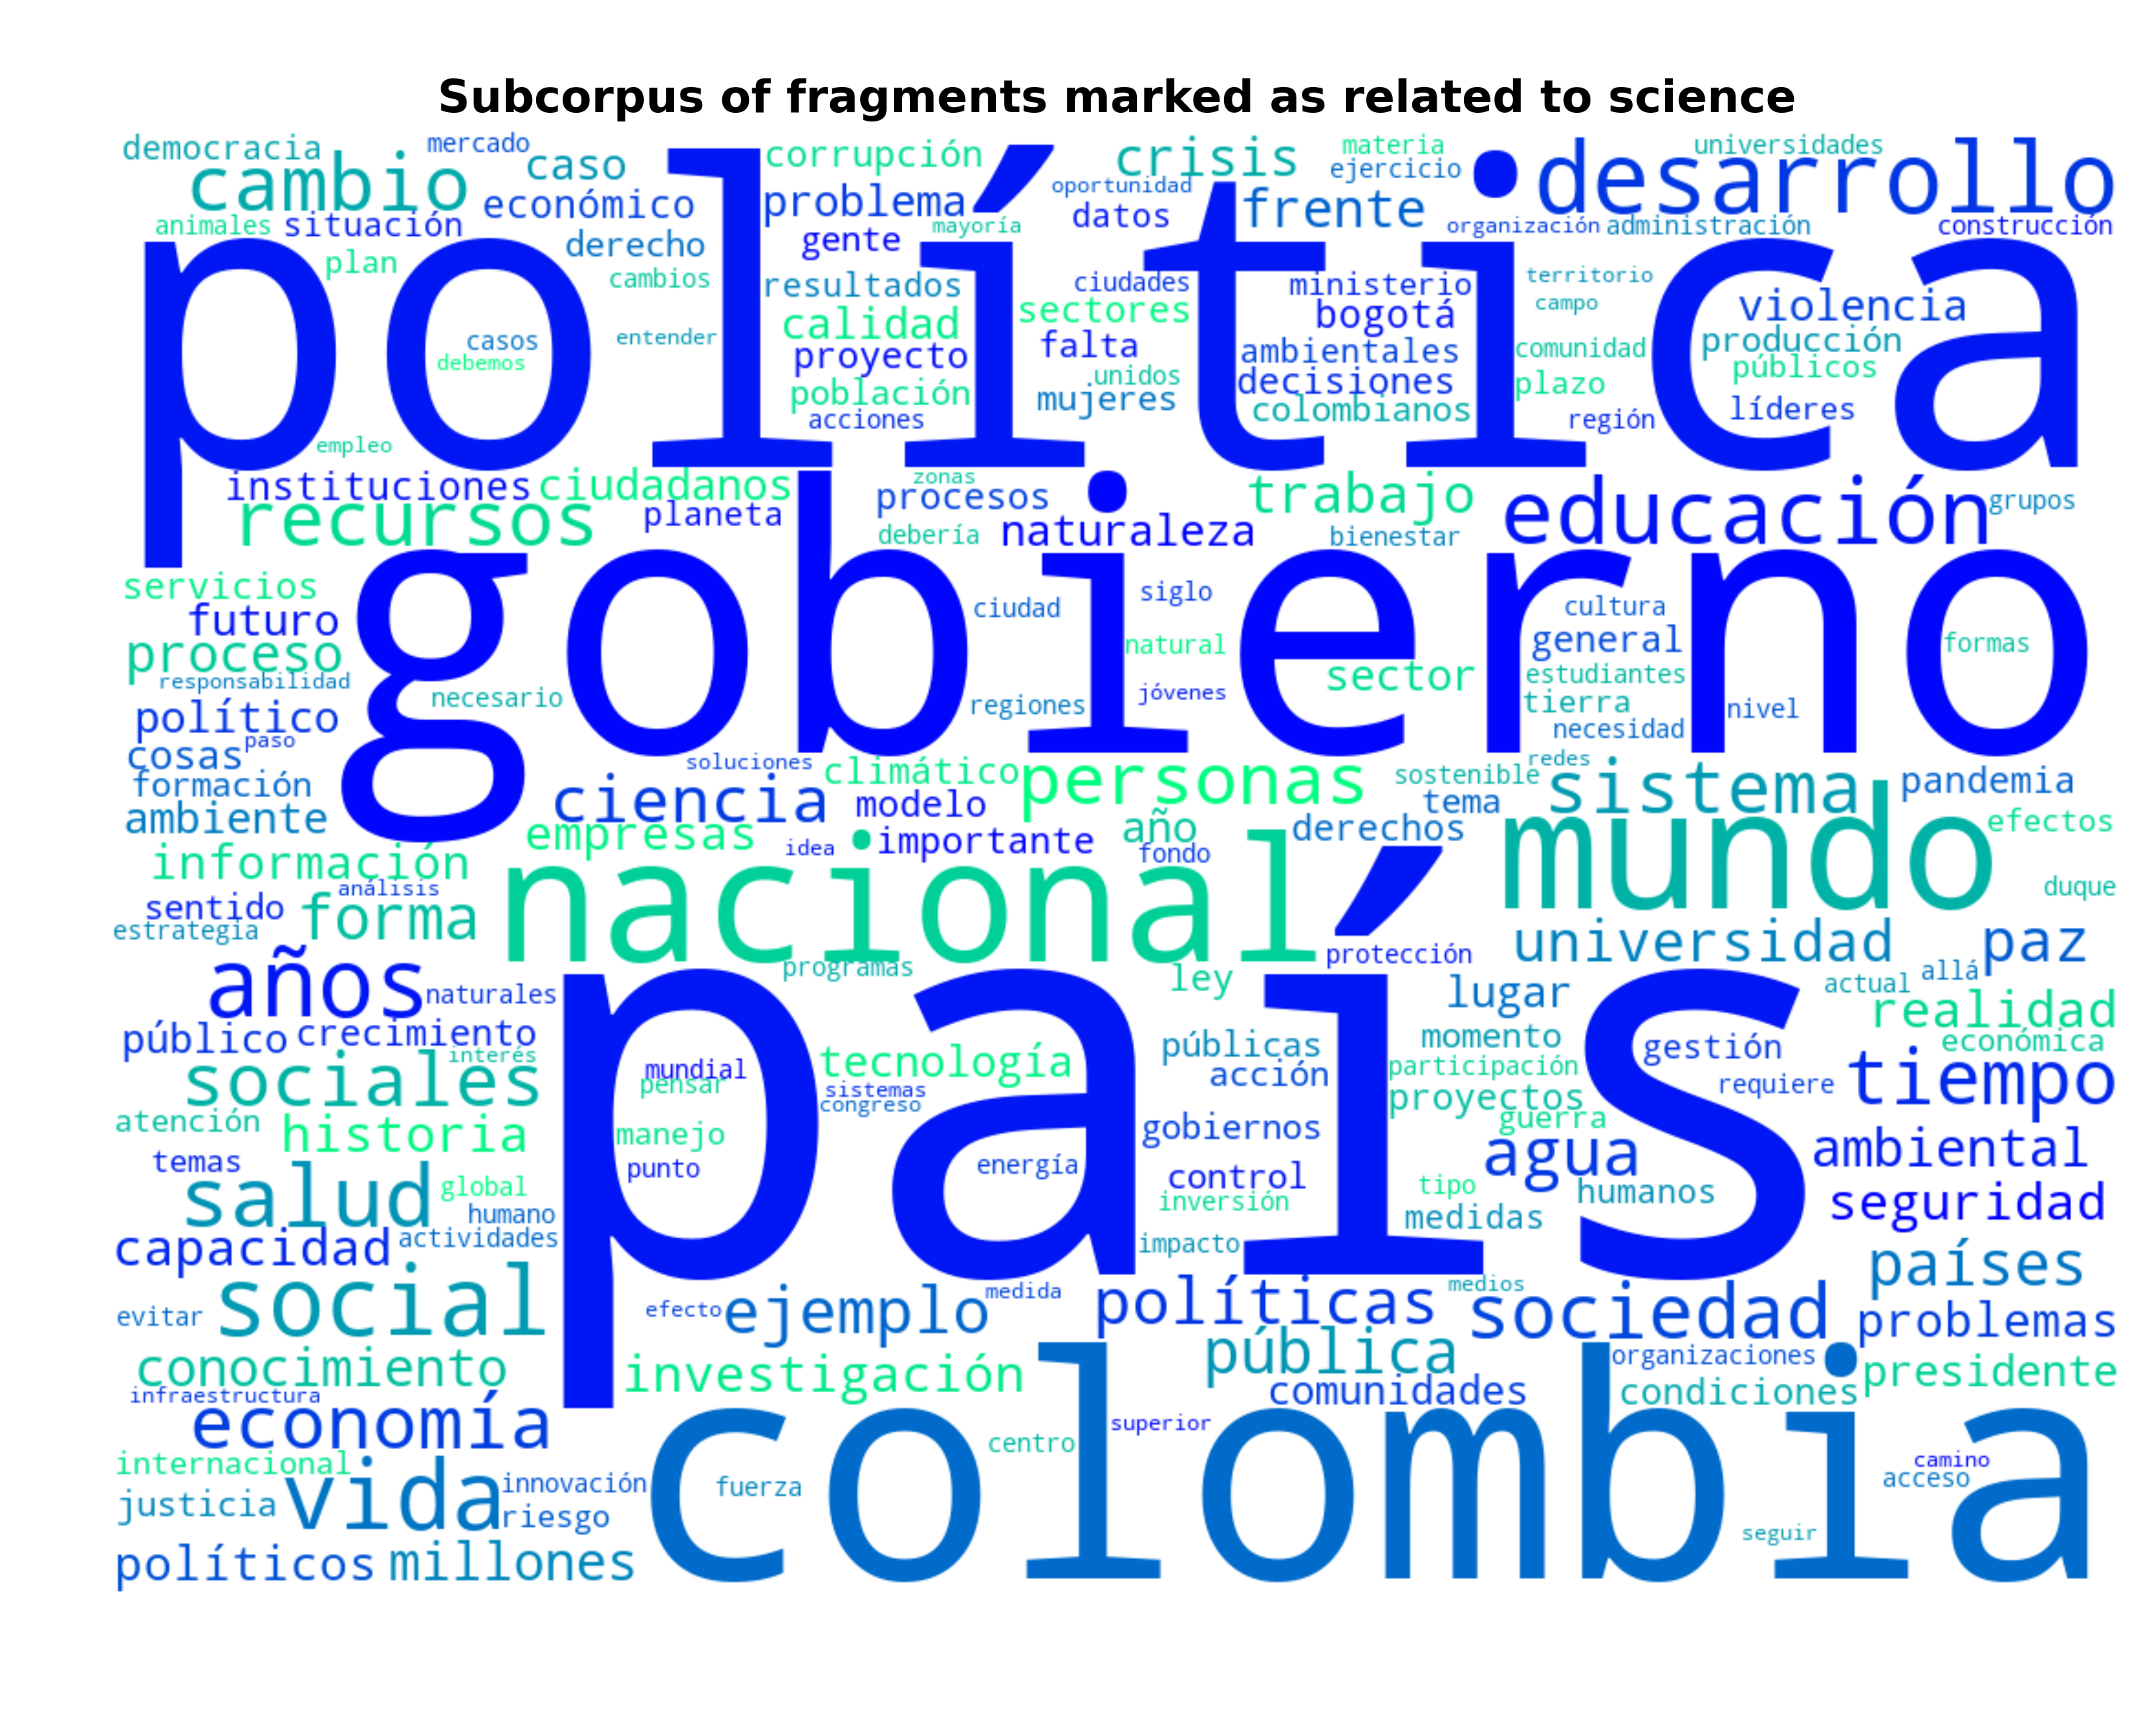
\includegraphics[width=\textwidth]{figures/nube_ciencia.png}
			\caption{Nube de palabras, fragmentos marcados como ciencia}
			\label{fig:nube_ciencia}
		\end{subfigure}
		\caption{Nubes de palabras}
		%\label{fig:resultados-clasificacion}
	\end{figure}
	


Figure~\ref{fig:dist_mensual_ciencia} shows, for each month in the analyzed period, the percentage of columns containing at least one effective mention of science relative to the total number of columns published in that month. This representation makes it possible to observe the temporal evolution of the presence of scientific discourse in public opinion. A notable increase can be observed in March and April 2020, the months with the highest proportion of mentions, suggesting a direct association between the intensification of scientific discourse and the onset of the COVID-19 pandemic.


	
	\begin{figure}[H]
		\centering
		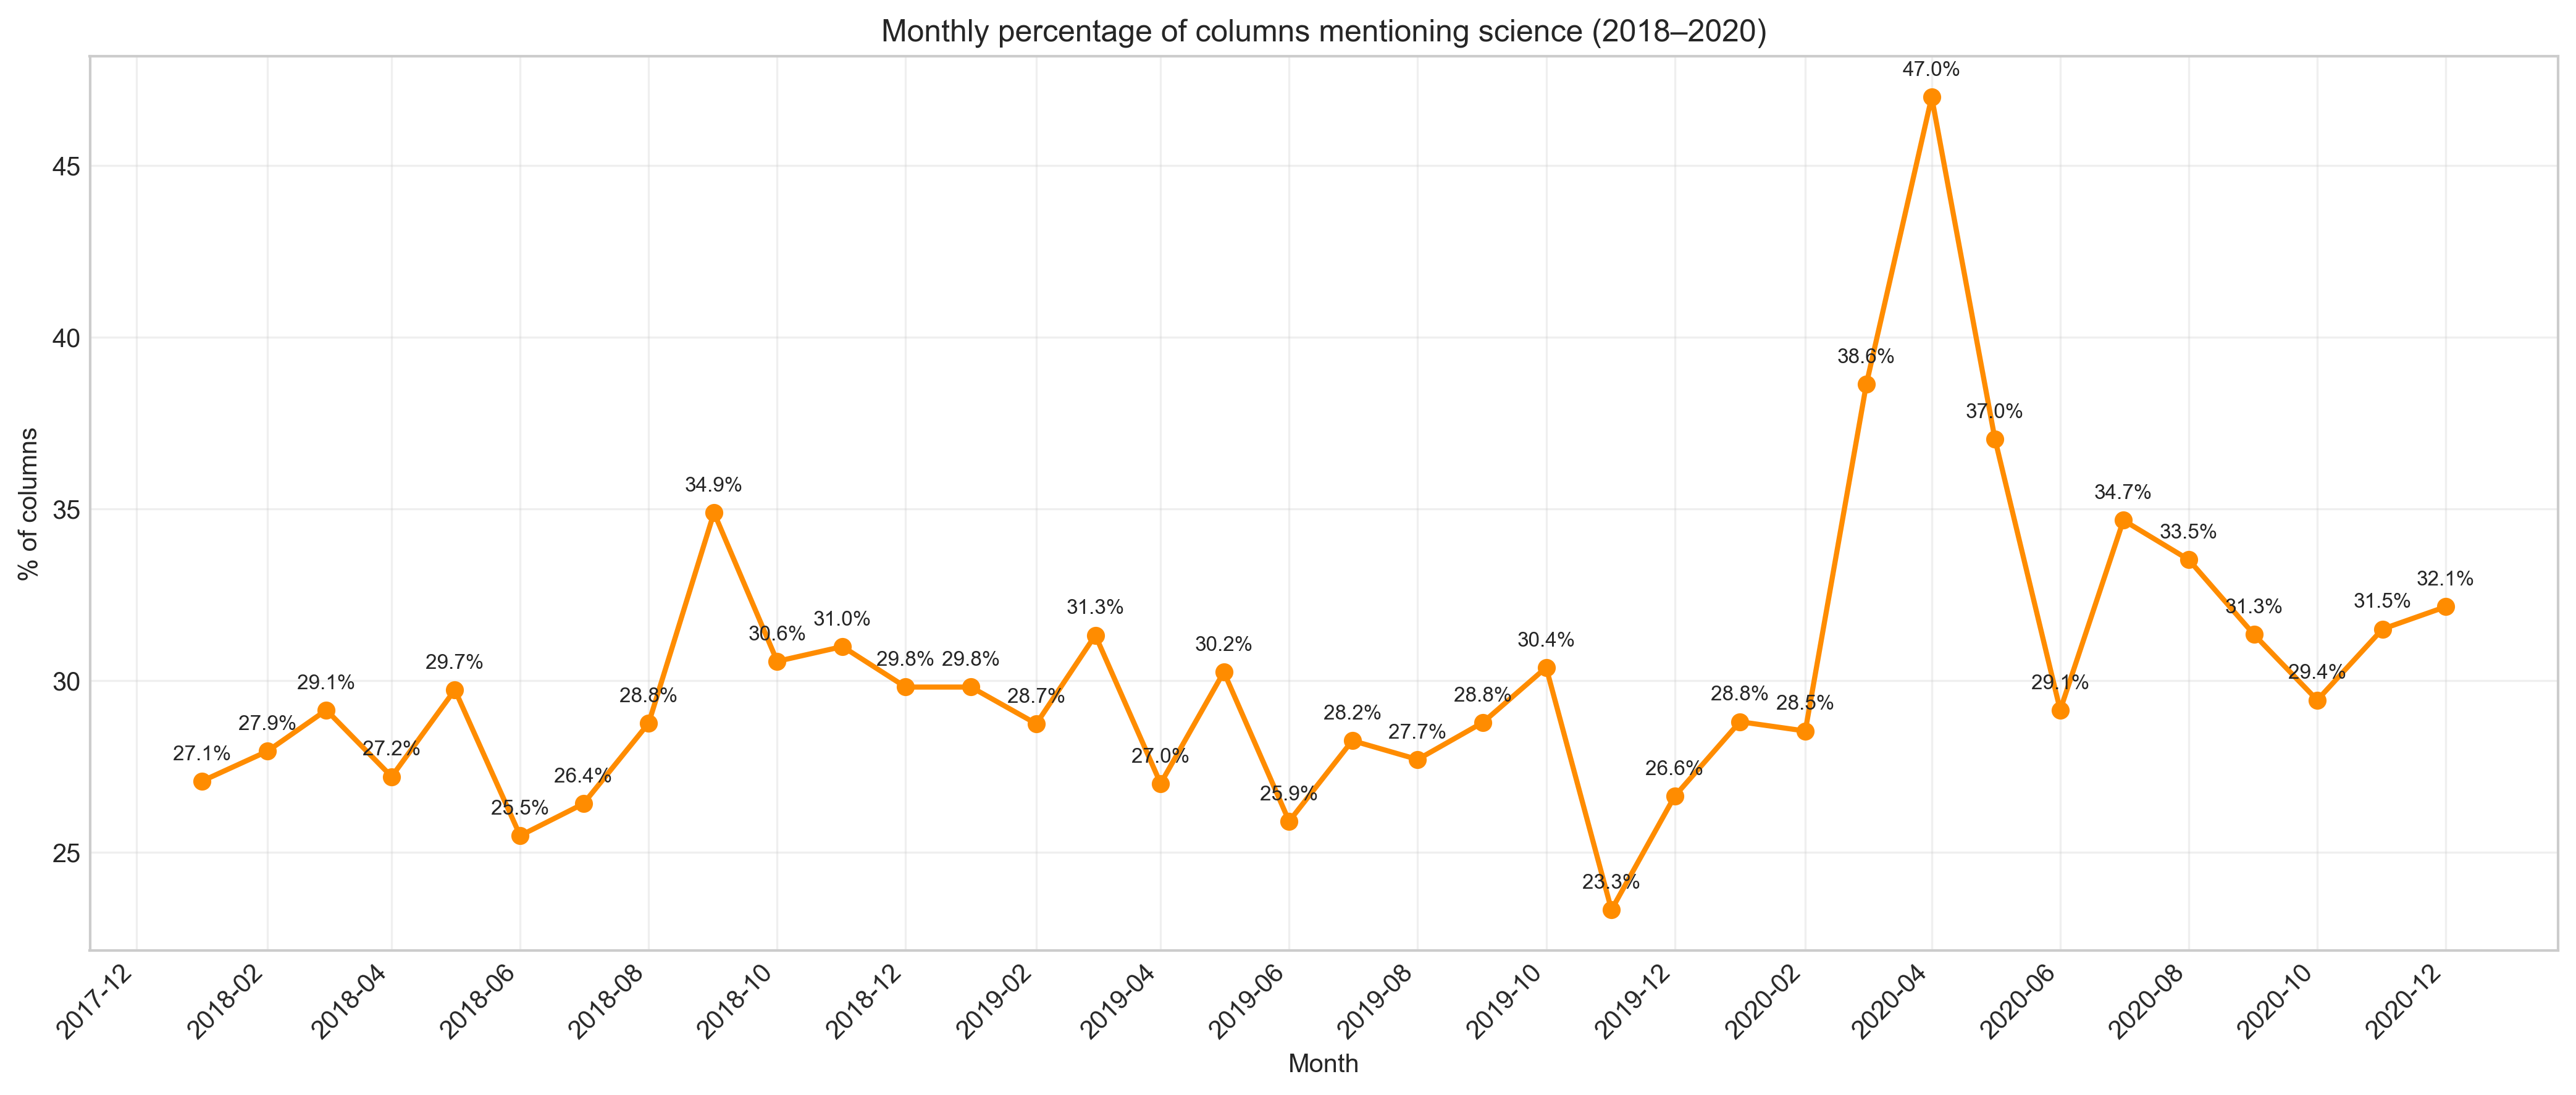
\includegraphics[width=0.95\textwidth]{figures/porcentaje_mensual_ciencia_linea.png}
		\caption{Distribución mensual de las columnas con menciones a la ciencia en porcentaje}
		\label{fig:dist_mensual_ciencia}
	\end{figure}
	
	
	
\subsection{Named Entity Recognition}


The ten most frequent entities by class (Person, Organization, and Location) are presented below, considering only those whose occurrence exceeds 30\% of the subcorpus of fragments with effective mentions of science. This criterion makes it possible to focus the analysis on the actors, institutions, and geographic spaces with the greatest centrality in the scientific discourse of opinion columns.

	
	

	\begin{table}[H]
		\centering
		\caption{Frecuencia comparativa de personajes en corpus general vs. corpus científico}
		\label{tab:ents_per}
		\footnotesize 

		\begin{tabular}{p{3cm}P{2.2cm}P{2.2cm}P{2.2cm}p{5cm}}
			\toprule
			\textbf{Entidad (PER)} & 
			\textbf{Frec. Corpus} & 
			\textbf{Frec. Ciencia} & 
			\textbf{\% Ciencia/ Corpus} & 
			\textbf{Descripción} \\
			\midrule
			Humboldt & 63 & 23 & 36 & Naturalista, geógrafo y explorador alemán, siglo XVIII y XIX. \\
			Newton & 25 & 9 & 36 & Físico inglés, siglos XVII y XVIII. \\
			Stephen Hawking & 41 & 16 & 39 & Científico y divulgador británico, siglos XX y XXI. \\
			Charles Darwin & 25 & 11 & 44 & Naturalista inglés, siglo XIX. \\
			Greta Thunberg & 50 & 16 & 32 & Activista ambiental sueca, siglo XXI. \\
			Ricardo Lozano & 15 & 7 & 46 & Geólogo y ex ministro de Ambiente y Desarrollo Sostenible de Colombia (2018). \\
			Mabel Torres & 13 & 7 & 53 & Científica colombiana y ex Ministra de Ciencia, Tecnología e Innovación de Colombia (2020) \\
			Wade Davis & 12 & 4 & 33 & Científico canadiense-colombiano. \\
			Dolly Montoya Castaño & 12 & 4 & 33 & Científica colombiana y ex rectora de la Universidad Nacional de Colombia. \\
			Carl Sagan & 10 & 5 & 50 & Astrónomo, astrofísico, divulgador estadounidense, siglo XX.\\
			
			\bottomrule
		\end{tabular}
	\end{table}
	
		\begin{table}[H]
		\centering
		\caption{Frecuencia comparativa de organizaciones en corpus general vs. corpus científico}
		\label{tab:ents_org}
		\footnotesize 
		
		\begin{tabular}{p{3cm}P{2.2cm}P{2.2cm}P{2.2cm}p{5cm}}
			\toprule
			\textbf{Entidad (ORG)} & 
			\textbf{Frec. Corpus} & 
			\textbf{Frec. Ciencia} & 
			\textbf{\% Ciencia/ Corpus} & 
			\textbf{Descripción} \\
			\midrule
			OCDE & 296 & 86 & 30 & Organización para la Cooperación y el Desarrollo Económico, organización internacional
			 \\
			Universidad Pedagógica Nacional & 117 & 55 & 47 & Universidad pública en Colombia \\
			Pontificia Universidad Javeriana & 103 & 33 & 32 & Universidad privada en Colombia. \\
			Ministerio de Agricultura & 111 & 33 & 30 & Ministerio de Colombia encargado del Sector Agropecuario, Pesquero y de Desarrollo Rural.  \\
			Colciencias & 74 & 47 & 63 & Anterior entidad encargada de promover las políticas públicas en ciencia, tecnología e innovación en Colombia. Reemplazada por Minciencias en 2019. \\
			Ministerio de Ambiente y Desarrollo Sostenible & 70 & 41 & 59 & Ministerio colombiano encargado de políticas en materia ambiental. \\
			Universidad de Massachusetts Amherst & 49 & 21 & 42 & Universidad pública y centro de investigación de Estados Unidos ubicada en Amherst, Massachusetts. \\
			Finagro & 44 & 15 & 34 & Fondo para el financiamiento del sector agropecuario, organización financiera en Colombia. \\
			IDEAM & 40 & 24 & 60 & Instituto de Hidrología, Meteorología y Estudios Ambientales de Colombia. \\
			FAO & 40 & 15 & 37 & Organización de las Naciones Unidas para la Alimentación y la Agricultura.\\
			
			\bottomrule
		\end{tabular}
	\end{table}
	
	\begin{table}[H]
		\centering
		\caption{Frecuencia comparativa de ubicaciones geográficas en corpus general vs. corpus científico}
		\label{tab:ents_loc}
		\footnotesize 
		\begin{tabular}{p{3cm}P{2.2cm}P{2.2cm}P{2.2cm}p{5cm}}
			\toprule
			\textbf{Entidad (LOC)} & 
			\textbf{Frec. Corpus} & 
			\textbf{Frec. Ciencia} & 
			\textbf{\% Ciencia/Corpus} & 
			\textbf{Descripción/Contexto} \\
			\midrule
			Amazonia & 306 & 112 & 37,21 & Región biogeográfica que comprende la selva tropical de la cuenca del Amazonas en Suramérica. \\
			Hidroituango & 127 & 46 & 36,22 & Proyecto hidroeléctrico en Antioquia, Colombia, sobre el río Cauca. \\
			Río Cauca & 93 & 33 & 32,58 & Segundo río más importante de Colombia, atraviesa la región andina. \\
			Orinoquia & 40 & 14 & 35,00 & Región natural de Colombia y Venezuela, también conocida como Llanos Orientales. \\
			Río Bogotá & 31 & 16 & 51,61 & Río que atraviesa la sabana de Bogotá, con importantes problemas de contaminación. \\
			Sabana & 28 & 13 & 46,43 & Referencia a la Sabana de Bogotá, altiplano en la cordillera Oriental. \\
			Parques Nacionales Naturales (PNN) & 35 & 15 & 33,33 & Sistema de áreas protegidas de Colombia, dependiente del Ministerio de Ambiente. \\
			Mar Caribe & 20 & 7 & 35,00 & Mar abierto tropical del océano Atlántico, baña las costas norte de Colombia. \\
			Mocoa & 18 & 9 & 50,00 & Ciudad capital del departamento de Putumayo, Colombia, en la región amazónica. \\
			\bottomrule
		\end{tabular}
	\end{table}
	
	
	\subsection{Modelado de tópicos}
Inicialmente, este ejercicio de modelado de tópicos se realizó sobre el corpus completo, con el propósito de caracterizar la estructura temática general de las columnas de opinión antes de focalizar el análisis en el subcorpus de ciencia. Para ello, se ejecutó el modelo variando el parámetro \textit{num\_topics}, que define el número máximo de tópicos que pueden estimarse. Cada configuración del parámetro produce un modelo distinto, entendido aquí como una estructura específica de agrupación semántica en la que los fragmentos del corpus se distribuyen en un conjunto determinado de tópicos latentes.

Para cada modelo estimado se calculó la métrica de coherencia \textit{c\_v}, la cual evalúa el grado de consistencia semántica interna de los términos más representativos de cada tópico. En términos generales, valores más altos de coherencia indican que las palabras que definen un tópico tienden a coocurrir en el corpus, lo que suele asociarse con una mayor interpretabilidad desde el punto de vista humano. Reportar los resultados para distintas configuraciones permite comparar la calidad temática de los modelos y fundamentar la selección del número de tópicos más adecuado.

\textcolor{red}{Los resultados obtenidos se presentan en la Tabla~\ref{tab:coherence_topics}.}

\begin{table}[H]
	\centering
	\begin{tabular}{ccccc}
		\hline
		\textbf{num\_topics} & \textbf{num\_topics\_final} & \textbf{coherence\_c\_v} & \textbf{\% outliers} \\
		\hline
		auto & 63 & 0.681289 & 0.0 \\
		60   & 59 & 0.671076 & 0.0 \\
		30   & 29 & 0.652175 & 0.0 \\
		40   & 39 & 0.635335 & 0.0 \\
		20   & 19 & 0.545472 & 0.0 \\
		10   & 9  & 0.480771 & 0.0 \\
		\hline
	\end{tabular}
	\caption{Resultados del modelado de tópicos para distintos valores del parámetro \textit{num\_topics}}
	\label{tab:coherence_topics}
\end{table}

El número de tópicos finales es menor en una unidad respecto al valor inicialmente definido por el parámetro, ya que al aplicar la reducción de \emph{outliers} se elimina el tópico que agrupa los documentos considerados atípicos. Se observa que, en general, al aumentar el número máximo de tópicos, el valor de coherencia tiende a incrementarse, lo que sugiere una mayor homogeneidad semántica dentro de cada agrupación. En particular, cuando el modelo determina automáticamente el número de tópicos, se obtienen 63 tópicos finales y el mayor valor de coherencia entre las configuraciones evaluadas.

		
Manteniendo el modelo de 63 tópicos, en la tabla \ref{tab:bertopic_coherence_top} se presentan los 10 tópicos con mayor porcentaje de documentos agrupados, junto con el valor de coherencia calculado para cada uno y sus respectivas palabras representativas. En conjunto, estos 10 tópicos concentran el 70\% de los fragmentos analizados.
		
		\begin{table}[H]
			\centering
			\small
			\begin{tabularx}{\textwidth}{c c c X}
				\hline
				\textbf{Topic} & \textbf{Coherence  ($c_v$)} & \textbf{Percentage (\%)} & \textbf{Keywords} \\
				\hline
				0  & 0.5509 & 40.06 & presidente, gobierno, duque, paz, país, uribe, colombia, política, años, petro \\
				2  & 0.8437 & 5.58  & economía, impuestos, crecimiento, ingresos, fiscal, empresas, tasa, empleo, pib, déficit \\
				1  & 0.7322 & 5.27  & pandemia, virus, salud, coronavirus, covid19, mundo, cuarentena, medidas, crisis, personas \\
				3  & 0.8185 & 4.25  & educación, estudiantes, universidad, universidades, calidad, formación, superior, nacional, profesores, colegios \\
				4  & 0.8427 & 3.34  & mujeres, mujer, hombres, sexual, violencia, género, sexo, feminismo, acoso, sexuales \\
				7  & 0.6890 & 2.53  & redes, información, datos, facebook, medios, sociales, comunicación, personas, internet, twitter \\
				8  & 0.7879 & 2.23  & hectáreas, rural, deforestación, tierras, agricultura, productores, agropecuario, cultivos, \textcolor{green}{000}, desarrollo \\
				5  & 0.8642 & 2.13  & fútbol, jugadores, equipo, juego, equipos, copa, selección, deporte, gol, mundial \\
				20 & 0.5990 & 2.05  & corrupción, corruptos, públicos, consulta, anticorrupción, lucha, funcionarios, recursos, país, política \\
				6  & 0.8998 & 1.61  & cocina, comida, comer, restaurante, plato, sabores, arroz, platos, sabor, casa \\
				\hline
			\end{tabularx}
			\caption{Top tópicos de BERTopic con coherencia por tópico ($c_v$), porcentaje de documentos y palabras representativas}
			\label{tab:bertopic_coherence_top}
		\end{table}
		
		El mismo procedimiento fue aplicado a los fragmentos clasificados como menciones a la ciencia. 
		
		\begin{table}[H]
			\centering
			\begin{tabular}{c c c c}
				\hline
				\textbf{num\_topics} & \textbf{num\_topics\_final} & \textbf{Coherence $c_v$} & \textbf{\% Outliers} \\
				\hline
				20   & 19 & 0.695491 & 0.0 \\
				40   & 28 & 0.695162 & 0.0 \\
				auto & 26 & 0.694176 & 0.0 \\
				30   & 28 & 0.681233 & 0.0 \\
				60   & 27 & 0.678842 & 0.0 \\
				10   & 9  & 0.622583 & 0.0 \\
				\hline
			\end{tabular}
			\caption{Resultados de BERTopic para distintos valores de \texttt{num\_topics}, especifico ciencia}
			\label{tab:bertopic_nr_topics_ciencia}
		\end{table}
		
		En este caso, el mejor modelo entre los evaluados fue el de 20 tópicos, de acuerdo con la métrica utilizada. Para este modelo, los resultados se presentan en la Tabla \ref{tab:topics_ciencia}. Asimismo, se observa que el 90\% de los documentos se concentró en los 10 primeros tópicos, lo que indica una alta concentración temática en un subconjunto reducido de tópicos.
		
		\begin{table}[H]
			\centering
			\small
			\begin{tabularx}{\textwidth}{c c c X}
				\hline
				\textbf{Topic} & \textbf{Coherence ($c_v$)} & \textbf{Percentage (\%)} & \textbf{Keywords} \\
				\hline
				1  & 0.493785 & 25.62 & política, gobierno, paz, país, seguridad, violencia, político, políticos, justicia, colombia \\
				0  & 0.460526 & 21.69 & salud, mundo, vida, pandemia, tiempo, ciencia, personas, virus, años, crisis \\
				3  & 0.574302 & 11.42 & economía, desarrollo, crecimiento, recursos, país, sector, gobierno, política, fiscal, innovación \\
				2  & 0.782987 & 9.61  & educación, universidad, formación, universidades, estudiantes, nacional, calidad, investigación, conocimiento, superior \\
				4  & 0.784604 & 6.56  & ambiental, ambientales, conservación, ambiente, biodiversidad, sostenible, desarrollo, deforestación, bosques, ecosistemas \\
				5  & 0.799532 & 4.79  & climático, cambio, planeta, global, calentamiento, incendios, mundo, climática, clima, temperatura \\
				8  & 0.504077 & 2.79  & datos, información, encuestas, acceso, transparencia, resultados, personas, medios, ejemplo, pública \\
				7  & 0.686045 & 2.75  & agua, río, aguas, lluvia, ríos, cauca, barrios, obras, bogotá, país \\
				9  & 0.919135 & 2.02  & energía, combustibles, fósiles, energías, carbón, renovables, solar, energética, petróleo, gas \\
				10 & 0.724657 & 1.83  & mujeres, hombres, mujer, género, femenino, violencia, personas, vida, femenina, sexo \\
				\hline
			\end{tabularx}
			\caption{Top tópicos de BERTopic con coherencia por tópico ($c_v$), porcentaje de documentos y palabras representativas, específico para menciones a ciencia}
			\label{tab:topics_ciencia}
		\end{table}
		
		
		
	\subsection{Análisis de vocabulario con POS-tagging}

Se extrajeron los verbos, adjetivos y sustantivos del corpus mediante técnicas de \emph{POS-tagging} y se calcularon sus frecuencias. En total, se identificaron aproximadamente 10 mil verbos, 18 mil adjetivos y 30 mil sustantivos distintos. En el corpus completo, el verbo más frecuente es \textit{tener}, el adjetivo más frecuente es \textit{social} y el sustantivo más frecuente es \textit{país}. Estas mismas palabras encabezan también las listas de frecuencia en el subcorpus de fragmentos con mención efectiva a la ciencia.

Dado que el 11.6\% de los fragmentos del corpus fueron clasificados como menciones científicas (véase sección \ref{sec:ident_menciones}), se seleccionaron aquellas palabras cuya proporción de ocurrencia en el subcorpus de ciencia supera ese porcentaje. Este criterio permite identificar términos con una presencia relativamente mayor en el discurso científico en comparación con el corpus general. A partir de este filtro se obtuvo el conjunto final de palabras analizadas en esta sección.



\begin{table}[H]
	\centering
	\begin{tabular}{lrrr}
		\toprule
		\textbf{Verbo} & \textbf{Frecuencia total} & \textbf{Frecuencia ciencia} & \textbf{Proporción ciencia} \\
		\midrule
		articular     & 175 & 79 & 0.45 \\
		mitigar       & 208 & 68 & 0.33 \\
		contaminar    & 200 & 63 & 0.32 \\
		gestionar     & 188 & 57 & 0.30 \\
		actualizar    & 122 & 37 & 0.30 \\
		deforestar    & 67  & 26 & 0.39 \\
		posibilitar   & 77  & 24 & 0.31 \\
		apalancar     & 54  & 22 & 0.41 \\
		planificar    & 43  & 20 & 0.47 \\
		capacitar     & 46  & 20 & 0.43 \\
		dinamizar     & 62  & 20 & 0.32 \\
		armonizar     & 47  & 19 & 0.40 \\
		maximizar     & 62  & 19 & 0.31 \\
		optimizar     & 39  & 18 & 0.46 \\
		cuantificar   & 47  & 18 & 0.38 \\
		almacenar     & 47  & 18 & 0.38 \\
		talar         & 39  & 17 & 0.44 \\
		\bottomrule
	\end{tabular}
	\caption{Frecuencia y proporción de verbos en el subcorpus de ciencia}
	\label{tab:verbos_ciencia}
\end{table}


\begin{table}[H]
	\centering
	\begin{tabular}{lrrr}
		\toprule
		\textbf{Adjetivo} & \textbf{Frecuencia total} & \textbf{Frecuencia ciencia} & \textbf{Proporción ciencia} \\
		\midrule
		ecosistémico & 65   & 53  & 0.82 \\
		invernadero  & 100  & 68  & 0.68 \\
		silvestre    & 133  & 81  & 0.61 \\
		hídrico      & 107  & 65  & 0.61 \\
		forestal     & 173  & 105 & 0.61 \\
		ambiental    & 1530 & 910 & 0.59 \\
		climático    & 984  & 584 & 0.59 \\
		renovable    & 149  & 84  & 0.56 \\
		fósil        & 196  & 110 & 0.56 \\
		ecológico    & 322  & 180 & 0.56 \\
		científico   & 959  & 507 & 0.53 \\
		energético   & 227  & 119 & 0.52 \\
		biológico    & 183  & 87  & 0.48 \\
		sostenible   & 744  & 342 & 0.46 \\
		animal       & 188  & 84  & 0.45 \\
		\bottomrule
	\end{tabular}
	\caption{Frecuencia y proporción de adjetivos en el subcorpus de ciencia}
	\label{tab:adjetivos_ciencia}
\end{table}

\begin{table}[H]
	\centering
	\begin{tabular}{lrrr}
		\toprule
		\textbf{Sustantivo} & \textbf{Frecuencia total} & \textbf{Frecuencia ciencia} & \textbf{Proporción ciencia} \\
		\midrule
		agua          & 2586 & 971 & 0.38 \\
		ciencia       & 1575 & 858 & 0.54 \\
		conocimiento  & 1753 & 665 & 0.38 \\
		tecnología    & 1547 & 622 & 0.40 \\
		naturaleza    & 1537 & 480 & 0.31 \\
		impacto       & 1419 & 462 & 0.33 \\
		formación     & 1124 & 412 & 0.37 \\
		ambiente      & 1256 & 398 & 0.32 \\
		gestión       & 1164 & 380 & 0.33 \\
		planeta       & 1207 & 379 & 0.31 \\
		energía       & 968  & 363 & 0.38 \\
		innovación    & 604  & 333 & 0.55 \\
		bosque        & 701  & 326 & 0.47 \\
		bienestar     & 1051 & 321 & 0.31 \\
		área          & 1037 & 314 & 0.30 \\
		\bottomrule
	\end{tabular}
	\caption{Frecuencia y proporción de sustantivos en el subcorpus de ciencia}
	\label{tab:sustantivos_ciencia}
\end{table}

	
\section{Discussion}
	
The applied methods made it possible to identify and characterize elements of discourse related to science in Colombian opinion columns. Based on a natural language processing strategy and the use of the UNESCO Thesaurus as a conceptual framework, it was possible to detect textual fragments with varying degrees of association with science and to construct a specific subcorpus for further analysis.


However, this approach presents inherent limitations linked to the way the concept of science is operationalized through term lists and semantic similarity measures. In particular, the method may generate classification errors, both false positives and false negatives. In this regard, the maximum accuracy achieved (74\%) indicates acceptable performance for large-scale exploratory analysis, although it also underscores the need to interpret the results cautiously and to consider methodological improvements in future research, for example through larger validation sets or hybrid schemes combining automatic and manual annotation.


The distribution presented in Table~\ref{tab:res_fragmentos_subcategoria} reveals a marked thematic concentration: nearly half of the fragments containing mentions of science fall within the category Administration of science and research (43.97\%), followed by Pollution, disasters and safety (21.55\%). This pattern suggests that, in the analyzed opinion discourse, science appears primarily linked to its institutional and political dimension (funding, management, public policy) and to contexts of socio-environmental crisis and risk. In contrast, specific scientific disciplines (such as physical, chemical, or earth sciences) occupy a much less visible position.


This asymmetry indicates that science does not circulate in the public sphere as a balanced set of disciplinary knowledges, but rather as a field associated with conjunctural and institutional debates. Nevertheless, it should be considered that the Thesaurus categories differ in conceptual breadth, which may influence their relative frequency. Even so, the observed concentration consistently points to a public representation of science centered more on governance and critical situations than on specialized technical discussion.

This thematic pattern is reinforced when considering its temporal dimension. As shown in Figure~\ref{fig:dist_mensual_ciencia}, the highest peaks in the proportion of columns containing mentions of science occur in March and April 2020, coinciding with the onset of the COVID-19 pandemic. In April 2020, the maximum value of the analyzed period is reached, evidencing a substantial increase in the public visibility of science. During these months, science and scientists assumed a central place in public debate, particularly in relation to governmental decisions, health measures, and risk management.


Regarding the actors and organizations mentioned in fragments associated with science (see Tables~\ref{tab:ents_per}, \ref{tab:ents_org}, \ref{tab:ents_loc}), the named entity recognition results show a predominance of widely recognized scientists, environmental activists, and Colombian scientists who have held political positions or ministerial offices. At the organizational level, prominent entities include international cooperation agencies linked to development, ministries responsible for science, environment, and sustainable development in Colombia, as well as national and international universities. This set of entities suggests that science, in opinion columns, appears closely tied both to state institutional structures and to academic and international networks, reinforcing its political and institutional character in the public sphere.


Based on the topic modeling applied to the subcorpus of fragments containing mentions of science (see Table~\ref{tab:topics_ciencia}), several clearly differentiated thematic axes were identified. The topic with the largest proportion (25.62\%) revolves around political and institutional categories (politics, government, peace, security), suggesting that science frequently appears embedded in broader public and governmental debates. The second largest topic (21.69\%) is associated with health and the pandemic (health, virus, crisis, science), confirming that the COVID-19 context played a central role in the visibility of scientific discourse. Relevant topics also emerge in connection with economic development (11.42\%) and education and research (9.61\%), indicating a link between science, innovation, and higher education. In the environmental domain, distinct topics are identified related to conservation and biodiversity (6.56\%), climate change (4.79\%), water resources (2.75\%), and energy (2.02\%), reinforcing the idea that environmental issues constitute a structural axis in the articulation between science and public opinion. Taken together, these results show that science does not appear exclusively as specialized technical content, but rather as a discursive resource that intersects with political, economic, educational, and environmental debates.


The vocabulary analysis reinforces and complements the findings of the topic modeling. In the case of adjectives, those associated with environmental and climate-related issues predominate, such as environmental, climatic, ecosystemic, or renewable, indicating that science is primarily characterized through ecological and sustainability-related concerns. The most representative nouns are linked to concepts such as technology, knowledge, nature, education, and management, suggesting a conception of science oriented both toward the production of knowledge and its practical application and institutional administration.


Regarding verbs, the high frequency of articulate is particularly noteworthy, pointing to a representation of science as an element that must be connected with other domains, such as public policy, economic development, education, or environmental management. Similarly, verbs such as mitigate play a central role in contexts related to reducing the effects of global warming, environmental degradation, or disease spread, evidencing a narrative in which science appears as a tool for addressing risks and crises. Finally, the recurrence of verbs such as manage, plan, and optimize reinforces the idea of science conceived not merely as the production of abstract knowledge, but as a strategic resource oriented toward decision-making, efficiency, and intervention in social and environmental problems.


Overall, these results suggest that, in Colombian opinion columns, science is predominantly represented from an instrumental and contextualized perspective, closely linked to critical junctures, environmental challenges, and governance processes, rather than as a set of abstract disciplines or decontextualized bodies of knowledge.

	
	
	\section{Limitaciones y consideraciones éticas}
	Cobertura mediática, sesgos de autoría/medio, ambigüedad semántica, cumplimiento de TOS/licencias, privacidad y reproducibilidad.
	
	\section{Reproducibilidad y datos}
	Enlace a repositorio (GitHub/OSF/Zenodo), scripts, versión de paquetes y \emph{conteiner} (\texttt{Dockerfile}) si aplica. 
	Describe estructura del repo y cómo reproducir figuras/tablas.
	
	\section{Conclusiones y trabajo futuro}
	Síntesis de aportes y próximos pasos (ampliar periodos, añadir encuestas, enriquecer anotaciones, análisis multilingüe, etc.).
	
	\section*{Agradecimientos}
	Reconocimientos a colaboradores, financiación, y fuentes de datos.
	
	% --- Bibliografía ---
	\bibliography{references}  % Crea un archivo references.bib con tus entradas
	

	
	
	% --- Apéndices (opcional) ---
	\appendix

	
\end{document}
